% ==================================================================================================== PART I
\part{Batch-level early exit}
\label{part:ee}

% ---------------------------------------------------------------------------------------------------- 1
\section{Problem statement}\label{sec:problem}

Early-exit networks attach small classifiers (\emph{exits}) after some layers, so an easy input can stop after a
few layers instead of all of them~\cite{deebert,pabee}. On a GPU, inputs are served in batches and a batch runs layer
by layer for all its members together. A single hard input, a \emph{straggler}, keeps the batch running to the last
layer, so early exits save compute (FLOPs) but little wall-clock time (Figure~\ref{fig:straggler}). DREX, GEEP and
Miao et al.\ report the same effect for batched BERT and LLM inference~\cite{drex,geep,miao}.

\begin{figure}[ht]
  \centering
  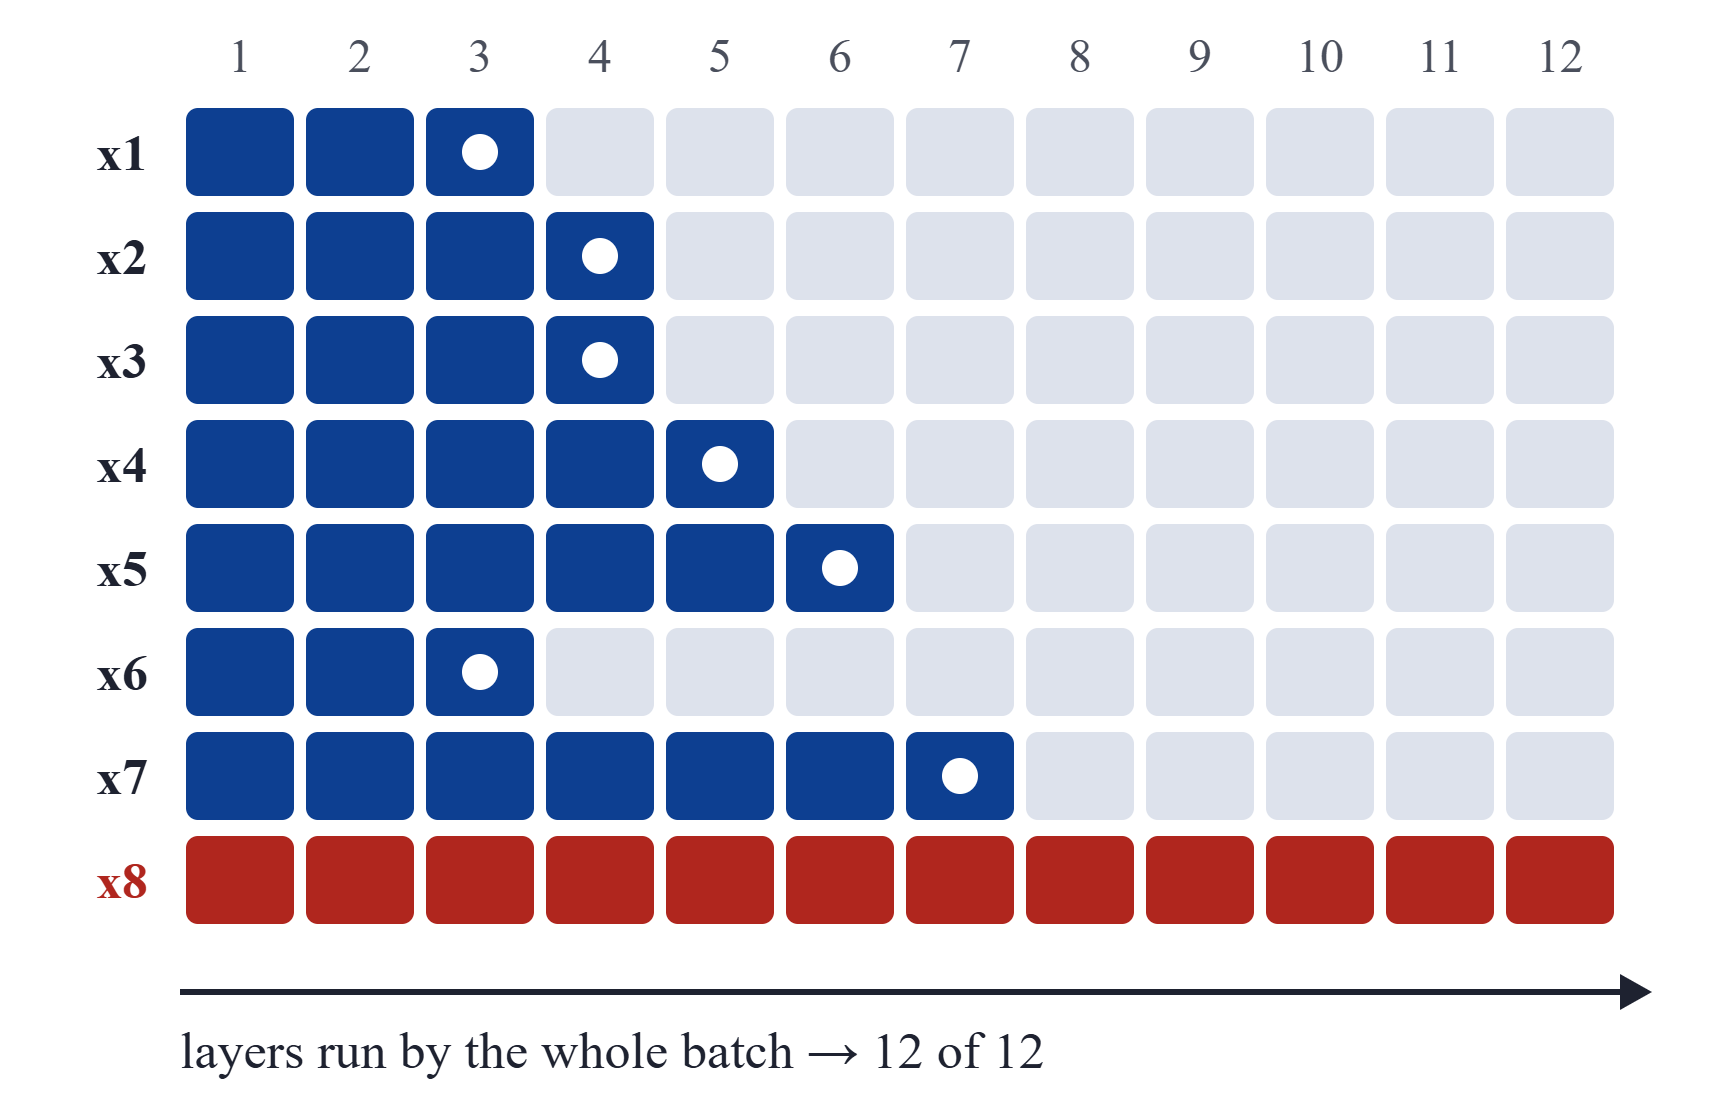
\includegraphics[width=0.62\textwidth]{fig/straggler.png}
  \caption{The straggler problem. One batch of 8 inputs through a 12-layer network. Blue: computed; grey: idle
  (the input already exited, $\circ$); red: the straggler. The mean exit is layer 5.5, yet the batch pays for all
  12 layers.}
  \label{fig:straggler}
\end{figure}

\paragraph{Cost model.} One layer run on the $n$ inputs still active costs $c(n)$. Exits sit after layers
$l_1<\dots<l_E=L$. Only a subset is evaluated, the \emph{exit plan} $S=\{s_1<\dots<s_m=E\}$, and each evaluated
exit costs $h$. Write $d_i$ for the layer of the $i$-th evaluated exit ($d_0=0$) and $n_i$ for the number of inputs
active on the layers between evaluated exits $i-1$ and $i$. If the batch ends at its $k$-th evaluated exit, its
latency is
\begin{equation}\label{eq:latency}
  T_{\text{batch}} \;=\; \sum_{i=1}^{k} \big[(d_i-d_{i-1})\,c(n_i) + h\big].
\end{equation}
Every layer up to the stopping depth is paid for, including layers whose exits are not in the plan; $h$ is paid only
for exits that are evaluated.

The first report assumed $c(n)=a+bn$ and described the regime by $\rho=a/(bn)$. When $\rho$ is small
(compute-bound), removing an exited input saves real time, so per-input exits work. When $\rho$ is large
(fixed-cost-bound), removing one input saves almost nothing and only stopping the whole batch saves time. That
picture stands, but Section~\ref{sec:cost} shows the affine form is a poor fit on a second GPU, so the method takes
the measured $c(n)$ directly.

\paragraph{Gap.} Existing batch-level rules are heuristics: Consensus waits until every input is confident, and
Majority and Greedy stop when half or one of them is~\cite{drex,miao}. None is derived from the cost. Apparate
chooses which exits to keep by their saving minus their overhead, but all inputs still run to the end of the model
and accuracy is monitored without a guarantee~\cite{apparate}. Risk-controlled early exit gives a guarantee, but for
per-input exits with no batch coupling~\cite{fastsafe}.

\paragraph{Setting, and what we do not compare against.} A batch is formed once, runs, and all its answers are
returned; the quantity of interest is the latency of that batch. The other way to deal with stragglers is to
rebatch: DREX regroups the inputs that continue past an exit into new batches with other requests waiting at that
depth, and E3 splits the model at its exits so that each part runs at a constant batch size~\cite{drex,e3}.
Rebatching needs other requests to regroup with, so it applies under sustained load; it does not apply to a fixed
offline batch, at low load, or when a batch has a latency deadline. The two are complementary, and this report has no
rebatching baseline, which is a limitation. Stopping a batch also has a cost that rebatching does not: the inputs
forced out are the hard ones, so the accuracy loss is not spread evenly. Section~\ref{sec:front} reports the loss on
hard inputs separately.

\paragraph{Security coupling.} A slowdown attacker crafts inputs that never become confident~\cite{sloth,lostpatience,falsesense}.
In a synchronous batch, such an input delays every co-batched user, not only itself.

\paragraph{Research questions.} Given the measured $c(n)$:
\begin{enumerate}
  \item When should a batch stop, and which exits are worth evaluating?
  \item Can the rule's parameters be set with a guarantee on accuracy, and learned online without labels?
  \item Can the damage from slowdown inputs be bounded without detecting them?
\end{enumerate}

% ---------------------------------------------------------------------------------------------------- 2
\section{Approach}\label{sec:approach}

\subsection{Batch-stopping rule for a measured cost}\label{sec:rule}
The objective for one batch is its mean accuracy minus $\lambda\cdot T_{\text{batch}}/F$, with $F$ the latency of
the full model at the same batch size. $\lambda$ has no unit: it is the accuracy we are willing to give up to save
one full-model latency. Let $g_j(e\to e')$ be the expected accuracy gain of carrying input $j$ from exit $e$ to a
later exit $e'$, estimated from a calibration table of $P(\text{correct at } e' \mid \text{confidence at } e)$. One
input contributes $1/B$ of the batch's mean accuracy, which is why its gain is divided by $B$. Input $j$ leaves alone
if
\begin{equation}\label{eq:indiv}
  \frac{g_j(e\to E)}{B} \;<\; \lambda\cdot\frac{[c(n)-c(n-1)]\,(L-l_e)}{F},
\end{equation}
and the remaining inputs $R$ stop together if no later evaluated exit is worth reaching:
\begin{equation}\label{eq:coll}
  \forall e'\in S,\ e'>e:\qquad \frac{1}{B}\sum_{j\in R} g_j(e\to e') \;<\;
  \lambda\cdot\frac{(l_{e'}-l_e)\,c(|R|) + m(e,e')\,h}{F},
\end{equation}
where $m(e,e')$ counts the evaluated exits after $e$ up to and including $e'$.

An individual exit saves only the marginal cost $c(n)-c(n-1)$; a collective stop saves all of $c(|R|)$. For the
affine cost these are $b$ and $a+b|R|$, which recovers the rule of the first report and its threshold ratio of about
$1/(1+\rho)$. For a cost with a floor the marginal cost is zero below the knee, so the rule switches from per-input
exits to whole-batch stopping inside a batch as it drains.

Two approximations are built in. Rule~\eqref{eq:indiv} prices the saving as if the input would otherwise run to
layer $L$ at today's marginal cost; when the batch later stops early the true saving is smaller, so~\eqref{eq:indiv}
overestimates it. Rule~\eqref{eq:coll} looks ahead to each later exit separately and uses only the current
confidences. Lookahead rules of this kind are optimal in the monotone case of optimal stopping~\cite{chow}, which
needs, among other conditions, gains that diminish with depth and a cost that is linear in $n$. On 13 November we
had not shown these conditions for a measured $c(n)$, and the floor-shaped cost of Section~\ref{sec:cost} violates
the linear one; Section~\ref{sec:theory} gives what we proved afterwards.

\subsection{Exit plan}\label{sec:plan}
The first rule evaluated every exit and paid $h$ for each. The plan $S$ is now a choice: any subset of the
intermediate exits, with the rule \eqref{eq:indiv}--\eqref{eq:coll} run on that subset. With one exit kept the plan
behaves like a unified exit; with all exits kept it is the earlier rule. The plan and $\lambda$ are chosen together
by replaying calibration traces under the measured $c(n)$ and $h$; this needs no GPU time.

\subsection{Certified selection}\label{sec:cert}
The first report chose the fastest setting whose accuracy on the tuning split was within one point of the full
model, and it then lost 0.8--2.5 points on held-out data. We now split the tuning data in two. On the first part each
method's candidates are reduced to a path ordered from safest to fastest. On the second part the path is tested in
order: for candidate $\theta$, the drop in accuracy against the full model is computed per batch on $K$ disjoint
batches, $Z_1,\dots,Z_K$, and $\theta$ is certified if a one-sided $t$-test rejects ``mean drop $>\alpha$'' at
level $\delta$. Testing stops at the first candidate that fails (fixed-sequence testing, as in
Learn-then-Test~\cite{ltt}); the fastest certified candidate is used. We use $\alpha=1$ point and $\delta=10\%$.
Batches, not inputs, are the unit, because a batch-level rule couples the inputs of a batch. The test treats the $K$
batch drops as independent draws from one distribution. That holds here because the batches are disjoint random
groups from one split, and it means the guarantee covers inputs from the same distribution only. The $t$-test is
also valid only for large $K$; Section~\ref{sec:tighten} tests finite-sample bounds. The certificate holds for the
batch size and cost it was computed for, and recomputing it for a new deployment is a replay on the CPU.

\subsection{Label-free, partial-feedback bandit (secondary)}\label{sec:bandit}
The bandit replaces ``correct'' with ``agrees with the full model'', which upper-bounds the accuracy loss. Feedback is
censored: once a batch stops, its deeper exits are never seen. Probe batches run to full depth with probability
$c\,t^{-1/3}$, the partial-monitoring rate for a revealing action~\cite{labeleff}. Prior bandits for early exit
tune per-input thresholds~\cite{ceebert,ucbee}.

\subsection{Bounded damage from slowdown inputs}\label{sec:robust}
The robust rule leaves the $m$ largest gains out of the collective sum in~\eqref{eq:coll}. A trimmed sum is
monotone, so for $k\le m$ slowdown inputs $K$ among clean inputs $C$,
\[
  TS_m(C) \;\le\; TS_m(C\cup K) \;\le\; TS_{m-k}(C), \qquad\text{hence}\qquad
  \operatorname{depth}(C\cup K;\,m) \;\le\; \operatorname{depth}(C;\,m-k)
\]
for every batch. The property is simple, and it bounds the damage without removing it: the batch can still run
deeper as $k$ grows.

\textbf{Scope of the proof.} The argument covers the collective stop~\eqref{eq:coll} with the trimmed sum, for a
fixed set of active inputs. It does not cover the per-input exits of rule~\eqref{eq:indiv}. Slowdown inputs stay in
the batch, so they change the number $n$ of active inputs and with it the marginal cost $c(n)-c(n-1)$ that decides
whether a clean input leaves. For the measured cost, which is only made non-decreasing, this marginal cost need not
be monotone in $n$, so the active set under attack is not ordered against the clean one. For the full rule the bound
is therefore an empirical property: Sections~\ref{sec:robust4} and~\ref{sec:robust5} check it on every tested batch, and that is
evidence, not a proof.

% ---------------------------------------------------------------------------------------------------- 3
\section{Experimental setup}\label{sec:setup}

\begin{table}[ht]
  \centering\small
  \resizebox{\textwidth}{!}{\begin{tabular}{@{}lllcl@{}}
    \toprule
    Model & Task & Exits after layer & Full-model acc. & Used in \\
    \midrule
    RoBERTa-base~\cite{roberta} & MNLI~\cite{mnli} & 2, 4, \dots, 12 & 87.8\% & server and local \\
    RoBERTa-base & QQP~\cite{glue} & 2, 4, \dots, 12 & 91.1\% & server and local \\
    ViT-B/16~\cite{vit} & CIFAR-100~\cite{cifar} & 2, 4, \dots, 12 & 93.3\% & server \\
    \makecell[l]{Qwen2.5-1.5B, Llama-3.1-8B\\(decoders)~\cite{qwen,llama}} & \makecell[l]{WikiText-103~\cite{wikitext}\\next token} & 6 exits & 49.9\%, 53.6\% & \makecell[l]{server\\(negative result)} \\
    \makecell[l]{Qwen2.5-1.5B,\\Llama-3.1-8B-Instruct\\(classifiers)} & MNLI, QQP & \makecell[l]{Qwen 4, 8, \dots, 28;\\Llama 8, 12, \dots, 32\\(7 exits)}
      & \makecell{Qwen 89.4, 90.1\%;\\Llama 90.9, 90.9\%} & server \\
    \bottomrule
  \end{tabular}}
  \caption{Models and tasks. Encoder backbones were fine-tuned jointly with their six exits (training details in
  Step~R\ref{st:train}). The decoders' exits were trained on a frozen backbone (13 November) and then with LoRA
  (Section~\ref{sec:llm}). The LLM classifiers train LoRA adapters (rank 16, $\alpha=32$) and one head per exit
  on the last prompt token (Step~R\ref{st:llm}); their accuracies are MNLI, QQP on the whole validation set.}
  \label{tab:models}
\end{table}

\paragraph{Server.} One RTX A6000. Three kinds of measurement were made on it, and they differ:
\begin{itemize}
  \item \textbf{Figure~\ref{fig:server}} (13 November): the trained checkpoints in fp16 on real inputs, in two
  execution modes, eager PyTorch and CUDA graphs (a compiled stack).
  \item \textbf{Tables~\ref{tab:t11}, \ref{tab:t12} and~\ref{tab:t12b}} (after 13 November): the replay method of
  the local GPU described next, that is, a random-weight fp32 network replaying the trained model's recorded
  decisions, eager only. Their first captions said ``trained checkpoint, real inputs''; that label was wrong and is
  corrected here.
  \item \textbf{Tables~\ref{tab:t15}--\ref{tab:t16}} (LLM classifiers): trained weights and real prompts, bf16,
  eager.
\end{itemize}

\paragraph{Local.} One GTX 1650 (4\,GB), fp32 (fp16 is about four times slower on this card). The trained
checkpoints are not on this machine. The timed network has the trained model's architecture and tensor shapes with
random weights; every layer, exit head, host synchronisation, batch compaction and policy call is executed and timed,
and the exit decisions and predictions are those recorded for the trained model on the same inputs. Accuracy is
therefore exact for the trained model and time is exact for this hardware. Sequence lengths 16 and 32 use decisions
recorded at length 128; they show how the same policies behave when per-input compute is smaller, and they are not a
claim about truncated inputs.

\paragraph{Protocol.} Each validation set is split in half. Parameters are chosen on the tuning half by certified
selection (Section~\ref{sec:cert}; 40\% for tables and candidate paths, 60\% for the test) and reported on the
held-out half. Local timing runs 1{,}920 held-out inputs per pass at lengths 16 and 32 (5 rounds) and 768 at length
128 (3 rounds), with policies interleaved within a round; we report the median over rounds of the paired speedup and
its range.

\paragraph{Baselines.} Per-sample threshold (DeeBERT-style), unified exit (SkipDecode-style~\cite{skipdecode}, one
head evaluated), Majority (as in DREX), a 150-trial random search over a 3-parameter collective rule, and the
per-sample threshold given the same exit-plan search as our rule (an Apparate-style selection of exits~\cite{apparate}).

% ---------------------------------------------------------------------------------------------------- 4
\section{Results up to 13 November}\label{sec:status}

This section is the ``Current status'' section of the progress report of 13 November. The cost-rule rows of
Table~\ref{tab:resplit} were regenerated on 26 November after a caching bug was fixed (Appendix~\ref{app:issues});
the 13 November values are given in brackets where they changed. Ten numbers in the 13 November text do not match
the committed result files; they are corrected here and marked with a footnote.

\subsection{Corrections to the first report}
The progress report opened its results with the claims of the first report that the new measurements
narrowed or withdrew. Table~\ref{tab:corrections} lists them with the evidence and the hardware it was measured on.
\begin{table}[H]
  \centering\small
  \begin{tabularx}{\textwidth}{@{}>{\raggedright\arraybackslash}p{4.2cm}X>{\raggedright\arraybackslash}p{2.3cm}@{}}
    \toprule
    First report said & What the evidence shows & Measured on \\
    \midrule
    The rule matches or beats the best heuristic in every cell & With CUDA graphs it is never the single fastest
      rule: unified exit wins at $B\le16$ on text, a random search ties or wins at $B\ge64$. At $B=8$ on MNLI it was
      the slowest rule (0.86\x) & Server, CUDA graphs \\
    1.41\x, 2.10\x, 1.46\x{} at $B=64$ within one accuracy point & Those were simulated and selected on the held-out
      split. The real-GPU runs lost 0.8--2.5 points on held-out data & Server, eager \\
    The simulator tracks the GPU within about 5\% & Only at $B\ge64$ in eager mode; at $B\le16$ off by 1--47\%
      depending on the policy\footnotemark, and it overestimates in graph mode & Server, both modes \\
    Every collective rule beats per-sample exits at $B\le16$ & True on MNLI and QQP, not on CIFAR-100 & Server, ViT \\
    Robustness costs no clean speedup & True at high $\rho$. At low $\rho$ on CIFAR-100 the robust rule reaches
      1.24\x{} against 1.46\x\footnotemark & Server, ViT \\
    Tuned parameters carry over between deployments (assumed) & Tested and false for every method: in simulation the
      rule broke the one-point budget in 29--31\% of transfers & Simulation, 3 tasks \\
    \bottomrule
  \end{tabularx}
  \caption{Claims of the first report that were narrowed or withdrawn.}
  \label{tab:corrections}
\end{table}
\addtocounter{footnote}{-1}%
\corrtext{the 13 November text said ``15--32\% off''. How that aggregate was computed was not recorded, and it cannot
be traced to a result file; the per-policy errors at $B\le16$ in the result files are 1--47\%.}%
\stepcounter{footnote}%
\corrtext{the 13 November text said 1.12\x; the committed result file is a 22 November rerun and gives 1.24\x.}

\subsection{No rule wins everywhere, and the winner flips with the deployment (server)}\label{sec:server}
\begin{figure}[ht]
  \centering
  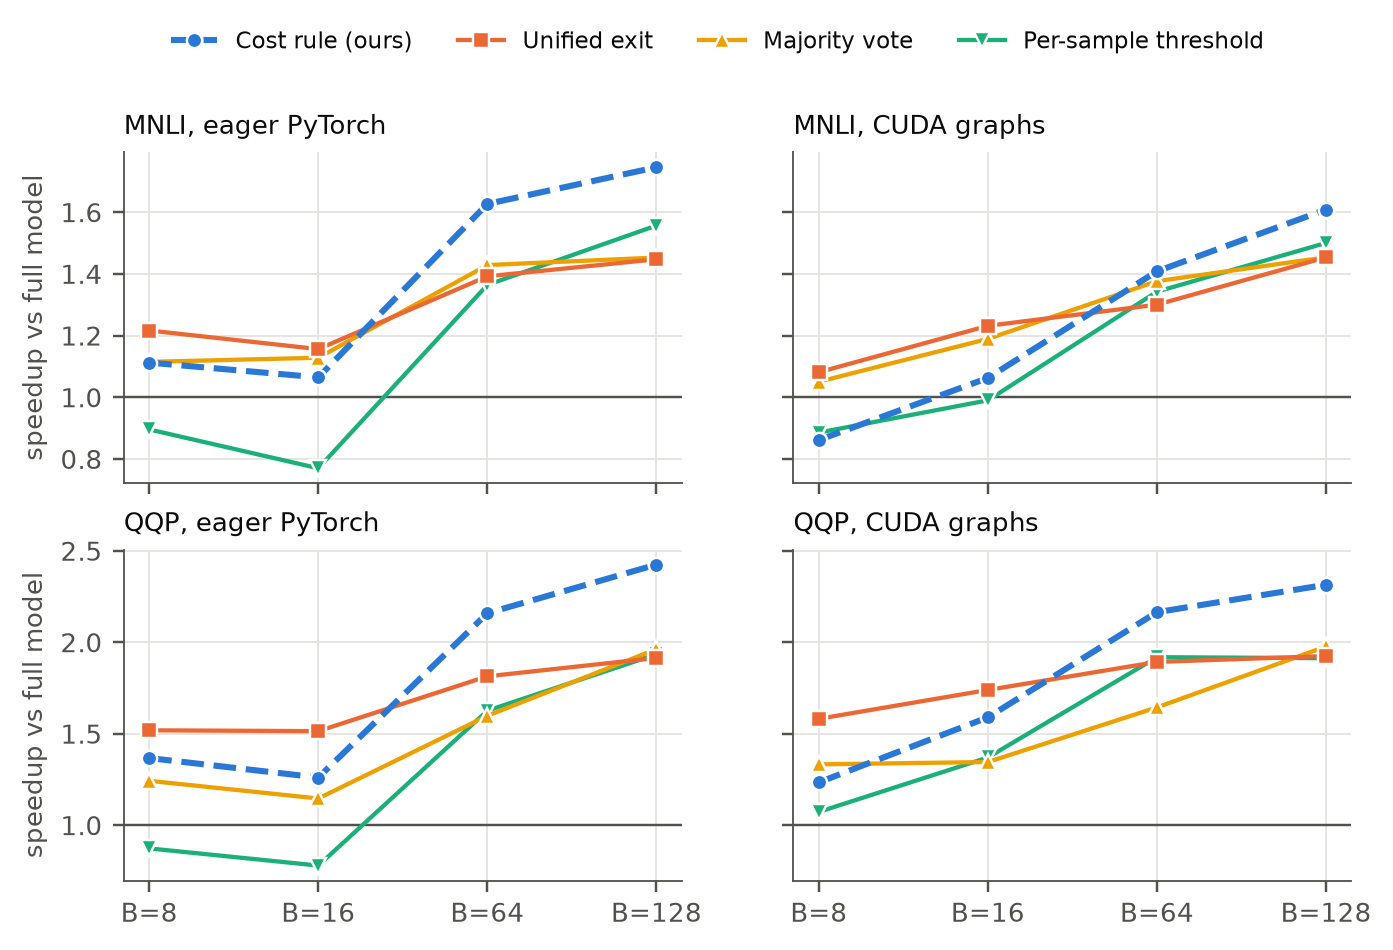
\includegraphics[width=0.92\textwidth]{fig/report2_server_speedups.png}
  \caption{Real wall-clock speedup against the full model on an RTX A6000, held-out split. Left: eager PyTorch.
  Right: CUDA graphs. These runs used the old selection protocol and are not accuracy-matched (on MNLI the cost rule
  lost 1.8--2.5 points, unified exit 0.8--0.9); Section~\ref{sec:server-cert} reruns them with certified selection.}
  \label{fig:server}
\end{figure}

Figure~\ref{fig:server} shows the server measurements. Three statements hold in both execution modes. Wait-for-all
early exit, which keeps exited inputs in the batch, is slower than no early exit (0.78--0.97\x). Per-sample exits fall
below 1\x{} at small batches on text (0.77--0.90\x{} eager, 0.89\x{} on MNLI with CUDA graphs). And the ordering of
rules changes between $B=8$ and $B=128$. Compiling cuts the fixed per-layer cost about six-fold, and the cause of the
small-batch loss changes with it: under CUDA graphs it is the exit heads, which alone cost 19\% of the runtime at
$B=8$ on MNLI (12\% on QQP).\corr{the 13 November text gave 19\% for both tasks; it is 19\% on MNLI and 12\% on QQP.}

\subsection{The cost is a floor followed by a linear part (GTX 1650)}\label{sec:cost}
\begin{figure}[ht]
  \centering
  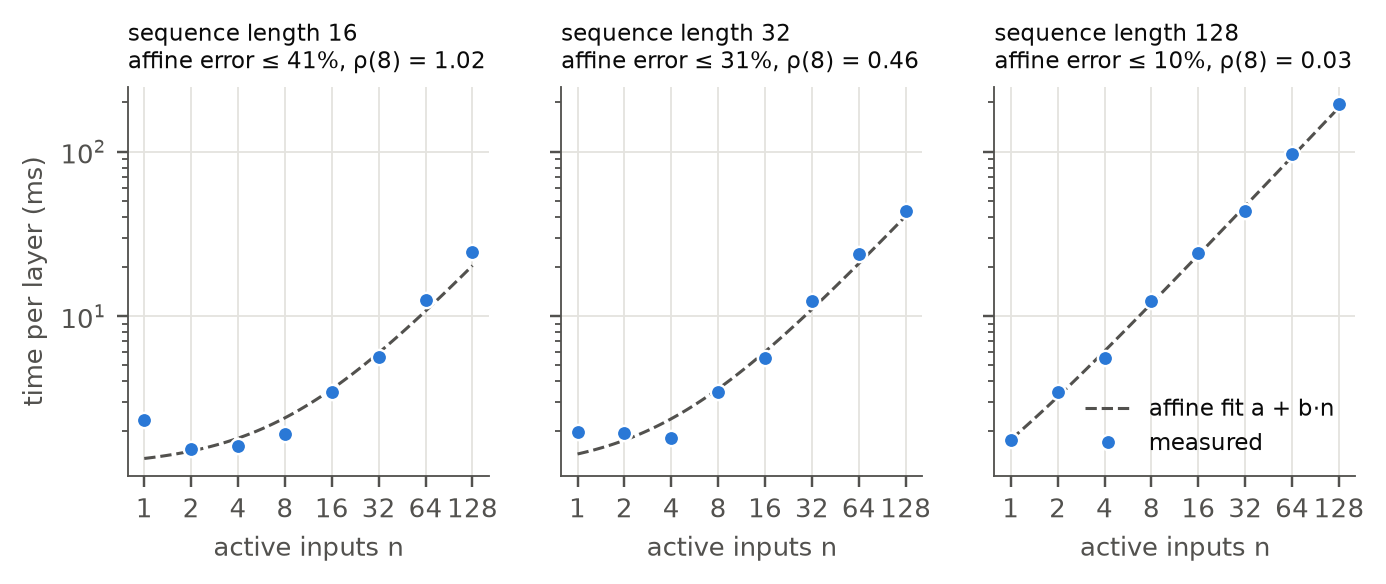
\includegraphics[width=0.92\textwidth]{fig/report2_cost_gtx1650.png}
  \caption{Measured time of one RoBERTa-base layer on a GTX 1650 (fp32) against the number of active inputs, at
  three sequence lengths, with the affine fit of the first report. Both axes are logarithmic.}
  \label{fig:cost}
\end{figure}

\begin{table}[ht]
  \centering\small
  \begin{tabular}{@{}lccccccc@{}}
    \toprule
    Sequence length & $c(1)$ ms & $c(8)$ ms & $c(64)$ ms & $h$ ms & $\rho$ at $n=8$ & $\rho$ at $n=64$ & \makecell{Affine fit,\\largest error} \\
    \midrule
    16  & 2.32 & 1.92  & 12.48 & 0.42 & 1.02 & 0.127 & 41\% \\
    32  & 1.97 & 3.46  & 24.00 & 0.42 & 0.46 & 0.058 & 31\% \\
    128 & 1.76 & 12.35 & 97.23 & 0.52 & 0.03 & 0.003 & 10\% \\
    \bottomrule
  \end{tabular}
  \caption{Per-layer cost and exit-head cost on the GTX 1650. File: \file{results/local\_cost\_cuda\_T\{16,32,128\}.json}.}
  \label{tab:cost}
\end{table}

A layer costs about 1.8\,ms however few inputs are active, and then grows in proportion to the number of tokens in
the batch. The knee is near 128 tokens: one input at length 128, four at length 32, eight at length 16. The affine
model is off by up to 41\% at short sequences. One GPU therefore covers both regimes: at length 128 it is
compute-bound at every batch size, and at length 16 with $B=8$ a per-input exit saves nothing. Policies below are
chosen with the measured table. The gain in predicting speedups is small, because a speedup is a ratio and errors
partly cancel: over the 126 policy runs timed in Section~\ref{sec:local} the table's median error is 1.3\% (largest
17\%), against 2.2\% (largest 15\%) for the affine fit applied to the same decisions. The floor matters for the
rule's decisions more than for the prediction.

\subsection{Exit plan and certified selection, real wall-clock (GTX 1650)}\label{sec:local}
\begin{figure}[ht]
  \centering
  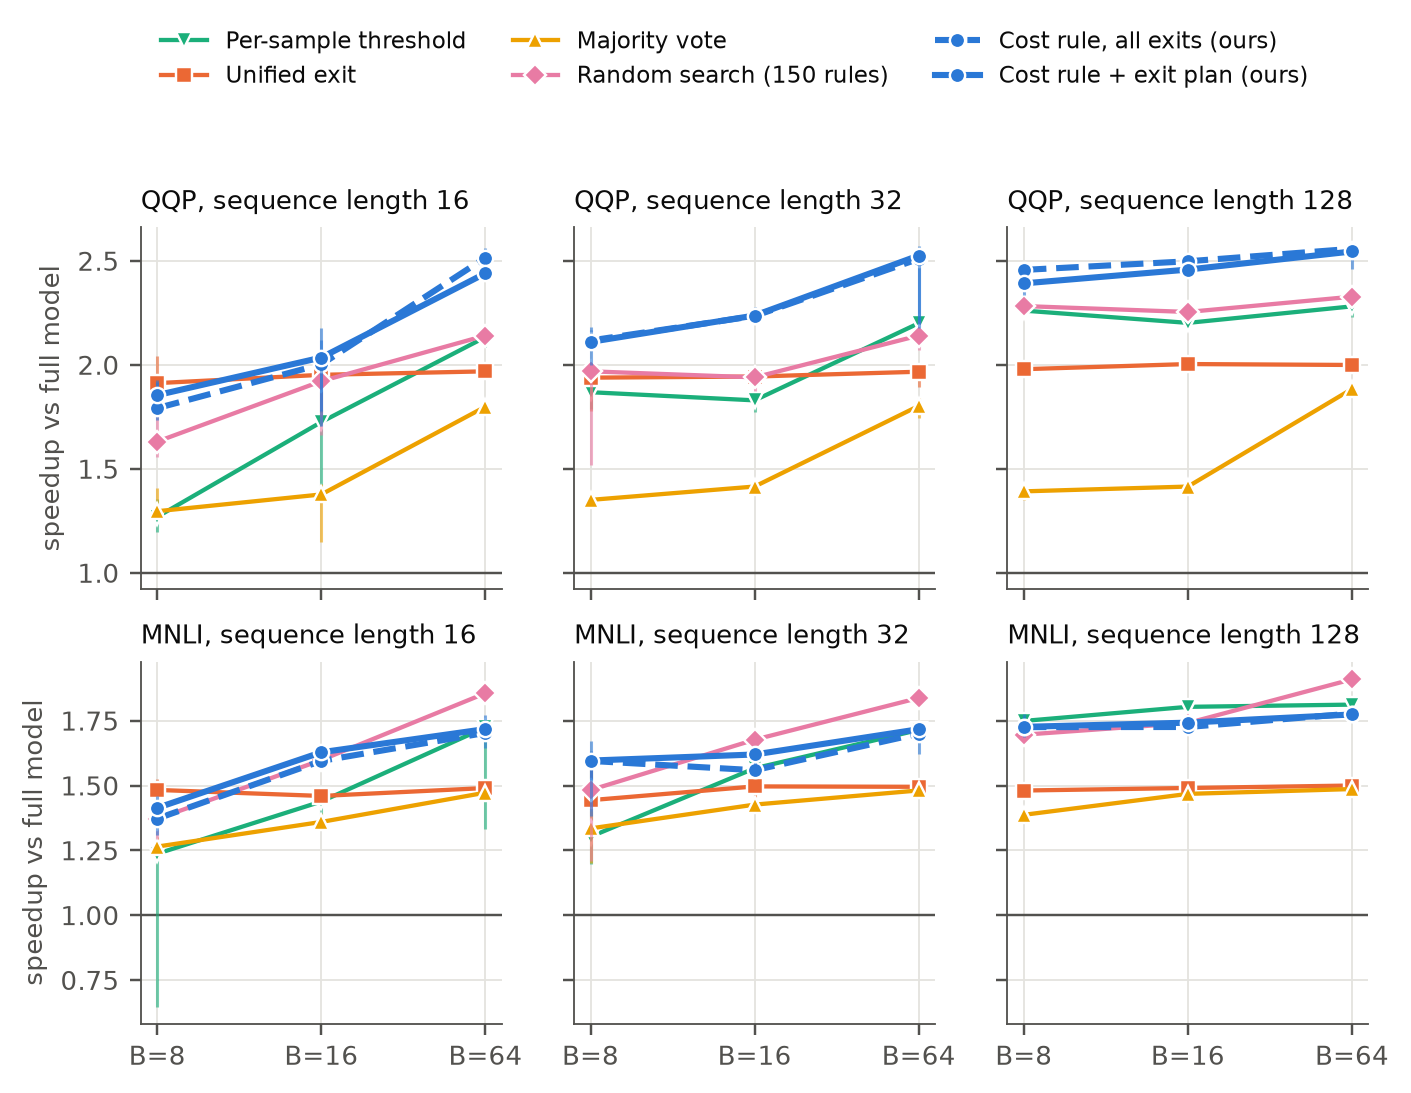
\includegraphics[width=0.86\textwidth]{fig/report2_local_speedups.png}
  \caption{Real wall-clock speedup on the GTX 1650 of the certified policy of each method, held-out inputs. Markers
  are the median over rounds; vertical bars are the range. Dashed blue: the cost rule with all exits; solid blue:
  with an exit plan.}
  \label{fig:local}
\end{figure}

\begin{table}[ht]
  \centering\footnotesize\setlength{\tabcolsep}{4pt}
  \begin{tabular}{@{}lccccccccc@{}}
\toprule
 & \multicolumn{3}{c}{sequence length 16} & \multicolumn{3}{c}{sequence length 32} & \multicolumn{3}{c}{sequence length 128} \\
\cmidrule(lr){2-4}\cmidrule(lr){5-7}\cmidrule(lr){8-10}
Policy & $B=8$ & $B=16$ & $B=64$ & $B=8$ & $B=16$ & $B=64$ & $B=8$ & $B=16$ & $B=64$ \\
\midrule
All heads, no exits & 0.93 & 0.96 & 0.99 & 0.96 & 0.97 & 0.99 & 0.99 & 0.99 & 1.00 \\
\midrule
Per-sample threshold & 1.27 & 1.73 & 2.13 & 1.87 & 1.83 & 2.20 & 2.26 & 2.20 & 2.28 \\
Threshold + exit plan & 1.86$^{*}$ & 1.92$^{*}$ & 2.15 & 1.93$^{*}$ & 1.90 & 2.19 & 2.27 & 2.20 & 2.30 \\
Unified exit & \textbf{1.91}$^{*}$ & 1.95$^{*}$ & 1.97$^{*}$ & 1.94$^{*}$ & 1.94$^{*}$ & 1.97$^{*}$ & 1.98$^{*}$ & 2.00$^{*}$ & 2.00$^{*}$ \\
Majority vote & 1.30 & 1.38 & 1.80 & 1.35 & 1.42 & 1.80 & 1.39 & 1.42 & 1.88 \\
Random search (150 rules) & 1.63 & 1.92 & 2.14 & 1.97 & 1.94 & 2.14 & 2.28 & 2.25 & 2.33 \\
\midrule
Cost rule, all exits \textit{(ours)} & 1.79 & 2.00 & \textbf{2.52} & \textbf{2.12} & \textbf{2.24} & 2.51 & \textbf{2.46} & \textbf{2.50} & \textbf{2.56} \\
Cost rule + exit plan \textit{(ours)} & 1.85 & \textbf{2.04} & 2.44 & 2.11 & \textbf{2.24} & \textbf{2.53} & 2.39 & 2.46 & 2.55 \\
\bottomrule
\end{tabular}

  \caption{QQP, GTX 1650, measured speedup of each method's certified policy. Bold: fastest in the column.
  $^{*}$ held-out accuracy drop above one point. File: \file{results/local\_time\_qqp\_cuda\_T\{16,32,128\}.csv}.}
  \label{tab:t04}
\end{table}

\begin{table}[ht]
  \centering\footnotesize\setlength{\tabcolsep}{4pt}
  \begin{tabular}{@{}lccccccccc@{}}
\toprule
 & \multicolumn{3}{c}{sequence length 16} & \multicolumn{3}{c}{sequence length 32} & \multicolumn{3}{c}{sequence length 128} \\
\cmidrule(lr){2-4}\cmidrule(lr){5-7}\cmidrule(lr){8-10}
Policy & $B=8$ & $B=16$ & $B=64$ & $B=8$ & $B=16$ & $B=64$ & $B=8$ & $B=16$ & $B=64$ \\
\midrule
All heads, no exits & 0.93 & 0.96 & 0.98 & 0.95 & 0.98 & 0.99 & 0.98 & 0.98 & 1.00 \\
\midrule
Per-sample threshold & 1.24$^{*}$ & 1.44$^{*}$ & 1.72$^{*}$ & 1.30$^{*}$ & 1.57$^{*}$ & 1.71$^{*}$ & \textbf{1.75}$^{*}$ & \textbf{1.80}$^{*}$ & 1.81$^{*}$ \\
Threshold + exit plan & 1.46 & 1.45 & 1.63 & 1.47 & 1.48 & 1.68 & 1.67 & 1.72 & 1.77 \\
Unified exit & \textbf{1.48} & 1.46 & 1.49 & 1.44 & 1.50 & 1.50 & 1.48 & 1.49 & 1.50 \\
Majority vote & 1.26$^{*}$ & 1.36 & 1.47 & 1.33$^{*}$ & 1.43 & 1.48 & 1.39$^{*}$ & 1.47 & 1.49 \\
Random search (150 rules) & 1.37 & 1.60$^{*}$ & \textbf{1.86}$^{*}$ & 1.48 & \textbf{1.68}$^{*}$ & \textbf{1.84}$^{*}$ & 1.70 & 1.74 & \textbf{1.91}$^{*}$ \\
\midrule
Cost rule, all exits \textit{(ours)} & 1.37$^{*}$ & 1.60$^{*}$ & 1.70$^{*}$ & \textbf{1.60}$^{*}$ & 1.56$^{*}$ & 1.70$^{*}$ & 1.73$^{*}$ & 1.73$^{*}$ & 1.78 \\
Cost rule + exit plan \textit{(ours)} & 1.41 & \textbf{1.63}$^{*}$ & 1.72$^{*}$ & \textbf{1.60}$^{*}$ & 1.62$^{*}$ & 1.72$^{*}$ & 1.73$^{*}$ & 1.74$^{*}$ & 1.77 \\
\bottomrule
\end{tabular}

  \caption{MNLI, same layout. File: \file{results/local\_time\_mnli\_cuda\_T\{16,32,128\}.csv}.}
  \label{tab:t05}
\end{table}

\begin{table}[ht]
  \centering\footnotesize
  \resizebox{\textwidth}{!}{\begin{tabular}{@{}lccccc@{}}
    \toprule
    Policy & \makecell{Mean speed rel.\\to the cell's best} & Worst cell & \makecell{Cells within\\3\% of the best}
      & \makecell{Cells over the 1-pt\\budget (held-out)} & \makecell{Largest held-out\\drop (pts)} \\
    \midrule
    Per-sample threshold        & 0.884 & 0.664 & 2 / 18  & 9 / 18 & 1.23 \\
    Threshold + exit plan       & 0.912 & 0.848 & 2 / 18  & 3 / 18 & 1.05 \\
    Unified exit                & 0.859 & 0.779 & 2 / 18  & 9 / 18 & 1.05 \\
    Majority vote               & 0.738 & 0.566 & 0 / 18  & 3 / 18 & 1.20 \\
    Random search (150 rules)   & 0.934 & 0.848 & 5 / 18  & 5 / 18 & 1.44 \\
    Cost rule, all exits (ours) & 0.970 & 0.917 & 11 / 18 & 8 / 18 & 1.31 \\
    Cost rule + exit plan (ours)& 0.975 & 0.925 & 11 / 18 & 7 / 18 & 1.28 \\
    \bottomrule
  \end{tabular}}
  \caption{Summary over 2 tasks \x{} 3 batch sizes \x{} 3 sequence lengths (18 timed cells; lengths 16 and 32 change
  the timing only, Section~\ref{sec:setup}). Speed is relative to the fastest method of each cell. The methods are
  not at the same accuracy here: the fifth column differs by method, so this table is not a ranking.
  Section~\ref{sec:front} compares speed at matched accuracy.}
  \label{tab:summary}
\end{table}

Tables~\ref{tab:t04}--\ref{tab:summary} and Figure~\ref{fig:local} give the measurements. What they show:
\begin{itemize}
  \item \textbf{The regime flip reproduces on this GPU.} On QQP at sequence length 16 and $B=8$, the per-sample
  threshold reaches 1.27\x{} and a unified exit 1.91\x; at $B=64$ the threshold reaches 2.13\x{} and the unified exit
  1.97\x. At sequence length 128, where the GPU is compute-bound at every batch size, the threshold is ahead of the
  unified exit throughout.
  \item \textbf{The cost rule is close to the fastest method in every timed cell, but not at equal accuracy.} With
  an exit plan it is at most 7.5\% behind (MNLI, $B=64$, behind the random search) and within 3\% of the fastest in
  11 of 18 settings. The best baselines by this measure, the random search and the threshold with an exit plan, are
  15\% behind in their worst setting; the unified exit 22\%; the per-sample threshold 34\%; majority vote 43\%. These
  policies do not sit at the same held-out accuracy: the rule is over one point in 7 of 18 cells, majority vote and
  the threshold with a plan in 3. The numbers in this item are therefore not a ranking; Section~\ref{sec:front}
  compares the methods at matched accuracy.
  \item \textbf{On QQP} one of the rule's two variants is the fastest in eight of nine settings (2.52\x{} against
  2.15\x{} for the next method at length 16 and $B=64$, with ranges that do not overlap) and 3\% behind the unified
  exit in the ninth. Its held-out drop with a plan is 0.52--0.82 points.
  \item \textbf{On MNLI it is not the fastest.} A unified exit is 5\% ahead at length 16 and $B=8$, and the random
  search is 7--8\% ahead at $B=64$, as it was on the server.
  \item \textbf{The exit plan helps only a little here.} It raises the rule from 1.79\x{} to 1.85\x{} (QQP) and from
  1.37\x{} to 1.41\x{} (MNLI) at length 16 and $B=8$, and changes little elsewhere: on this GPU the five exit heads
  cost at most 7\% of the runtime. The plan's real test is the server under CUDA graphs, where they cost 19\%.
  \item \textbf{The accuracy budget is not met on MNLI's held-out half.} Policies were certified at one point on the
  tuning half, yet on the held-out half the rule with a plan loses 0.88--1.28 points (7 of 9 MNLI settings above one
  point), the per-sample threshold 1.21--1.23 in all nine, and the random search up to 1.44. On QQP the unified exit
  lands at 1.05 points in all nine settings. Every method shifts by a similar amount on MNLI, which suggests the two
  4{,}900-example halves differ; Section~\ref{sec:resplit} tests the procedure on random re-splits.
\end{itemize}
\textbf{Limits of this experiment.} Decisions are replayed from recorded traces on a randomly initialised network
(Section~\ref{sec:setup}); 12 of the 18 cells are the same recorded decisions timed at a shorter sequence length, so
the independent workloads are 2 tasks \x{} 3 batch sizes; one GPU; three to five timing rounds per setting, so a range
is shown and not a confidence interval. At $B=16$ and length 16 one noisy round widens the ranges and the top four
methods are tied there.

\subsection{Speed at matched accuracy, and where the accuracy loss lands (cost table, GTX 1650)}\label{sec:front}
\begin{figure}[ht]
  \centering
  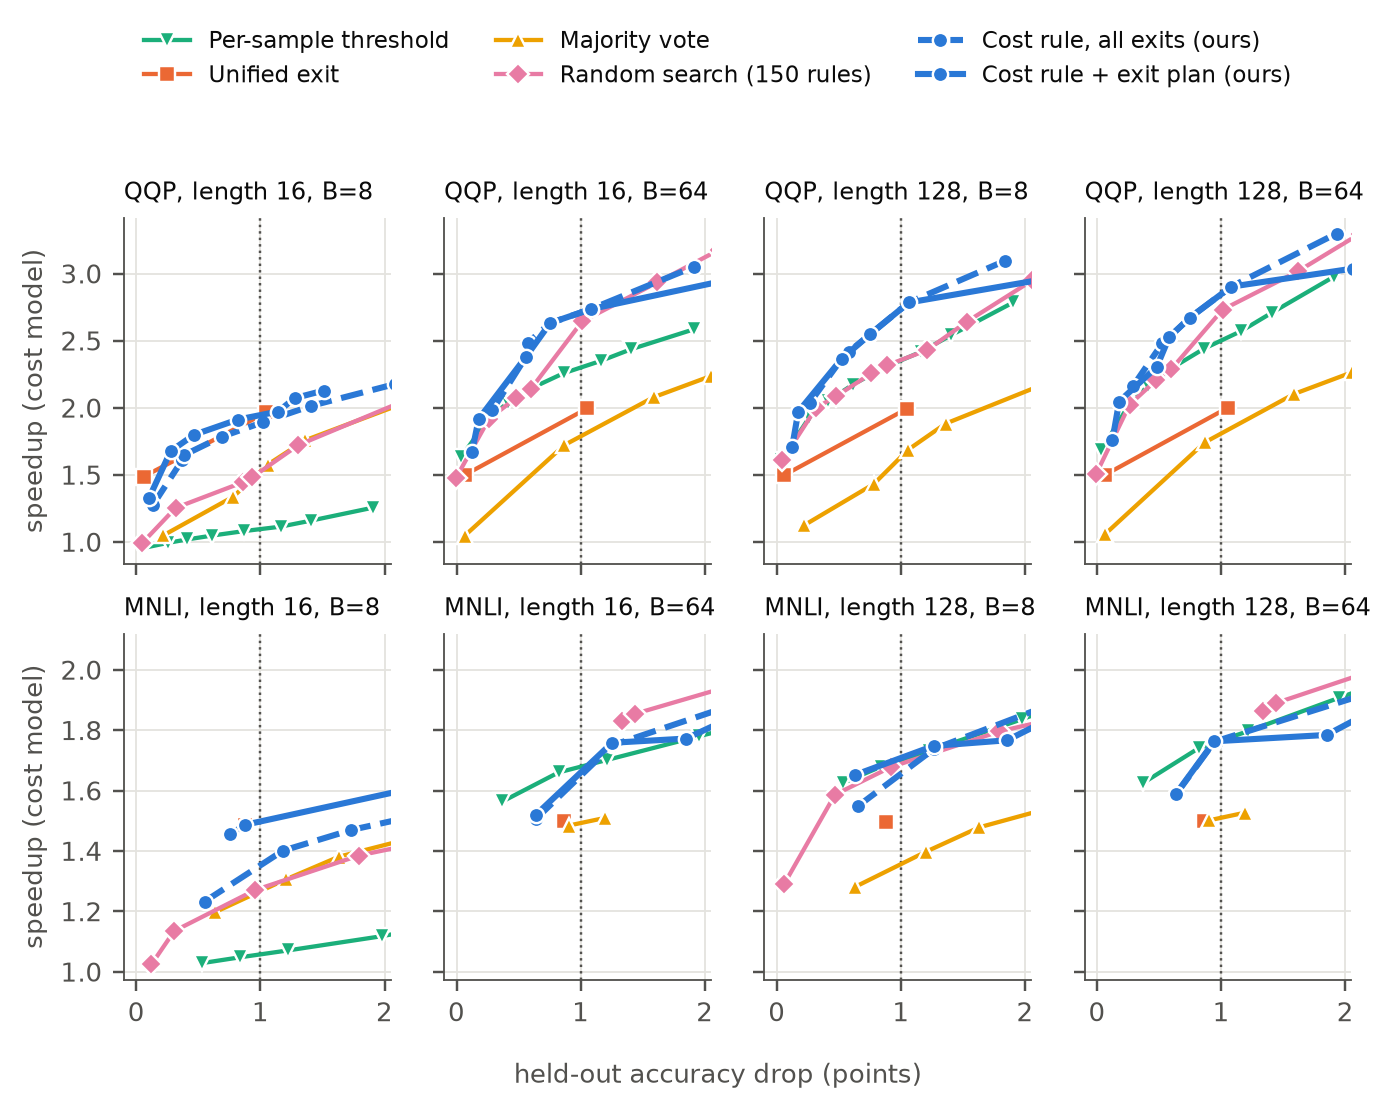
\includegraphics[width=0.82\textwidth]{fig/report2_front.png}
  \caption{Held-out accuracy drop against speedup. Each point is the policy that certified selection returns for one
  accuracy target between 0.25 and 3 points, scored once on the held-out half. Up and to the left is better. The
  dotted line is the one-point budget. Speedups are computed from the measured cost table, not timed.}
  \label{fig:front}
\end{figure}

\begin{table}[ht]
  \centering\small
  \begin{subtable}{\textwidth}\centering
    \begin{tabular}{@{}lcccccc@{}}
\toprule
 & \multicolumn{3}{c}{sequence length 16} & \multicolumn{3}{c}{sequence length 128} \\
\cmidrule(lr){2-4}\cmidrule(lr){5-7}
Policy & $B=8$ & $B=16$ & $B=64$ & $B=8$ & $B=16$ & $B=64$ \\
\midrule
Per-sample threshold & 1.08 & 1.48 & 2.26 & 2.30 & 2.32 & 2.44 \\
Threshold + exit plan & 1.88 & 1.89 & 2.16 & 2.26 & 2.29 & 2.35 \\
Unified exit & 1.49 & 1.49 & 1.50 & 1.50 & 1.50 & 1.50 \\
Majority vote & 1.34 & 1.45 & 1.72 & 1.43 & 1.51 & 1.74 \\
Random search (150 rules) & 1.48 & 1.89 & 2.14 & 2.32 & 2.36 & 2.29 \\
\midrule
Cost rule, all exits \textit{(ours)} & 1.78 & \textbf{2.13} & \textbf{2.63} & \textbf{2.55} & \textbf{2.48} & \textbf{2.67} \\
Cost rule + exit plan \textit{(ours)} & \textbf{1.91} & 2.08 & \textbf{2.63} & \textbf{2.55} & \textbf{2.48} & \textbf{2.67} \\
\bottomrule
\end{tabular}

    \caption{QQP. File: \file{results/local\_front\_qqp\_cuda\_T\{16,128\}.csv}.}\label{tab:t07}
  \end{subtable}\par\medskip
  \begin{subtable}{\textwidth}\centering
    \begin{tabular}{@{}lcccccc@{}}
\toprule
 & \multicolumn{3}{c}{sequence length 16} & \multicolumn{3}{c}{sequence length 128} \\
\cmidrule(lr){2-4}\cmidrule(lr){5-7}
Policy & $B=8$ & $B=16$ & $B=64$ & $B=8$ & $B=16$ & $B=64$ \\
\midrule
Per-sample threshold & 1.05 & 1.30 & \textbf{1.66} & \textbf{1.68} & 1.68 & 1.74 \\
Threshold + exit plan & 1.48 & 1.49 & 1.63 & 1.67 & 1.68 & 1.72 \\
Unified exit & \textbf{1.49} & 1.49 & 1.50 & 1.50 & 1.50 & 1.50 \\
Majority vote & 1.20 & 1.41 & 1.48 & 1.28 & 1.47 & 1.50 \\
Random search (150 rules) & 1.27 & 1.38 & -- & \textbf{1.68} & \textbf{1.69} & -- \\
\midrule
Cost rule, all exits \textit{(ours)} & 1.23 & 1.48 & 1.51 & 1.55 & 1.58 & \textbf{1.76} \\
Cost rule + exit plan \textit{(ours)} & \textbf{1.49} & \textbf{1.52} & 1.52 & 1.65 & -- & \textbf{1.76} \\
\bottomrule
\end{tabular}

    \caption{MNLI. File: \file{results/local\_front\_mnli\_cuda\_T\{16,128\}.csv}.}\label{tab:t08}
  \end{subtable}
  \caption{Speedup of each method's fastest policy whose held-out drop is at most one point (cost table, GTX 1650).
  Bold: best in the column. --: no such policy. (Tables 7 and 8 of the progress report.)}
  \label{tab:matched}
\end{table}

\begin{table}[ht]
  \centering\scriptsize\setlength{\tabcolsep}{3pt}
  \begin{tabular}{@{}lcccccccccccc@{}}
    \toprule
    & \multicolumn{3}{c}{QQP, length 16} & \multicolumn{3}{c}{QQP, length 128} & \multicolumn{3}{c}{MNLI, length 16} & \multicolumn{3}{c}{MNLI, length 128} \\
    \cmidrule(lr){2-4}\cmidrule(lr){5-7}\cmidrule(lr){8-10}\cmidrule(lr){11-13}
    Policy & all & hard 25\% & other & all & hard 25\% & other & all & hard 25\% & other & all & hard 25\% & other \\
    \midrule
    Per-sample threshold         & 0.61 & 1.03 & 0.47 & 0.61 & 1.03 & 0.47 & 1.22 & 0.57 & 1.44 & 1.22 & 0.57 & 1.44 \\
    Threshold + exit plan        & 0.90 & 3.06 & 0.18 & 0.61 & 1.03 & 0.47 & 0.89 & 2.07 & 0.50 & 0.97 & 0.57 & 1.10 \\
    Unified exit                 & 1.05 & 4.08 & 0.04 & 1.05 & 4.08 & 0.04 & 0.87 & 2.75 & 0.24 & 0.87 & 2.75 & 0.24 \\
    Majority vote                & 0.78 & 2.73 & 0.13 & 0.78 & 2.73 & 0.13 & 1.01 & 2.86 & 0.39 & 1.01 & 2.86 & 0.39 \\
    Random search (150 rules)    & 0.70 & 1.85 & 0.31 & 0.66 & 1.23 & 0.46 & 1.15 & 1.69 & 0.97 & 1.08 & 1.28 & 1.01 \\
    Cost rule, all exits (ours)  & 0.61 & 1.58 & 0.28 & 0.58 & 1.29 & 0.35 & 1.23 & 2.70 & 0.75 & 1.12 & 2.01 & 0.83 \\
    Cost rule + exit plan (ours) & 0.74 & 2.04 & 0.31 & 0.57 & 1.27 & 0.33 & 1.12 & 2.59 & 0.63 & 1.12 & 2.01 & 0.83 \\
    \bottomrule
  \end{tabular}
  \caption{Held-out accuracy drop in points at the one-point target, mean over $B=8,16,64$: all inputs, the hard
  quarter (lowest mean confidence over the five intermediate exits), and the rest. The rows of the threshold, the
  unified exit and majority vote are the same at both lengths because their certified parameters do not change with
  the cost table.}
  \label{tab:hard}
\end{table}

Tables~\ref{tab:t04}--\ref{tab:summary} compare one policy per method, and those policies differ in accuracy. Here
each method is run through certified selection at eight accuracy targets, which traces its accuracy--speed front on
held-out data (Figure~\ref{fig:front}). Table~\ref{tab:matched} reads each front at a held-out drop of at most one
point. Speedups in this section come from the measured cost table; over the timed runs of Section~\ref{sec:local}
the table's median error was 1.3\% and its largest 17\%.
\begin{itemize}
  \item \textbf{QQP:} the rule is ahead in all six settings, by 2--17\% over the best baseline (2.63\x{} against
  2.26\x{} at length 16 and $B=64$; 2.55\x{} against 2.32\x{} at length 128 and $B=8$).
  \item \textbf{MNLI: no advantage.} The rule is within 2\% of the best baseline in four of six settings and behind
  in two: 8.5\% behind the per-sample threshold at length 16 and $B=64$, and 6.5\% behind the random search at length
  128 and $B=16$. At length 128, where the GPU is compute-bound, the per-sample threshold is as fast as any
  batch-level rule.
  \item \textbf{The exit plan matters at small batches on the cost floor.} At length 16 and $B=8$ the rule without a
  plan reaches 1.23\x{} on MNLI and 1.78\x{} on QQP; with a plan, 1.49\x{} and 1.91\x. The threshold gains as much
  from the same plan search (1.05\x{} to 1.48\x{} on MNLI). On MNLI at this setting the plan keeps a single
  intermediate exit (layer 8) and is the same policy as the unified exit (both 1.49\x).
  \item \textbf{Why the plan variant is sometimes behind the rule with all exits.} The plan search uses every second
  value of $\lambda$, so it does not contain every all-exits policy, and selection on the tuning half can return a
  slower or a less accurate policy. The ``--'' in Table~\ref{tab:t08} arises this way: at length 128 and $B=16$ the
  selected plan policy has a held-out drop of 1.16 points at every target up to 2 points, so it has no point within
  one point.
  \item \textbf{What the derivation buys, and what it does not.} The rule without a plan has one parameter and 40
  candidates; the random search has three parameters and 150 candidates. With the plan search the rule has 620
  candidates, more than any baseline; the closest is the threshold with a plan (558). In five of the six QQP settings the rule
  without a plan is already ahead, so the lead there is not bought with a larger search. At length 16 and $B=8$ only
  the plan variant is ahead (1.91\x{} against 1.88\x{} for the threshold with a plan; 1.78\x{} without a plan), and
  the plan variant is not a cheaper search than the baselines. It does not buy transfer between deployments
  (Table~\ref{tab:corrections}). Whether it needs less calibration data is tested in Section~\ref{sec:tighten}.
  \item \textbf{The accuracy loss lands on hard inputs} (Table~\ref{tab:hard}). At the one-point target the rule
  loses 2.0--2.7 points on the hard quarter of MNLI and 1.3--2.0 on QQP, against 0.6 and 1.0 for the per-sample
  threshold. On MNLI the threshold takes its loss from the easier inputs (1.4 points on the other three quarters); on
  QQP its hard quarter also loses more than the rest (1.0 against 0.5). A unified exit is the most uneven (2.8 and
  4.1 points). This is a cost of any rule that stops a batch, ours included, and the one-point average hides it.
\end{itemize}
\textbf{Limits.} Speedups are from the cost table, not timed. Each front has at most eight points, and reading it at
``at most one point'' picks among them on held-out data, the same way for every method. MNLI's held-out half is
4{,}900 examples, so a difference of a few percent between two methods there is within noise we have not measured.

\subsection{Does the certificate hold on re-splits?}\label{sec:resplit}
\begin{table}[ht]
  \centering\footnotesize\setlength{\tabcolsep}{3.5pt}
  \begin{tabular}{@{}lllcccccc@{}}
    \toprule
    & & & \multicolumn{2}{c}{Over budget} & \multicolumn{2}{c}{Mean drop (pts)} & \multicolumn{2}{c}{Speedup (cost model)} \\
    \cmidrule(lr){4-5}\cmidrule(lr){6-7}\cmidrule(lr){8-9}
    Task & $B$ & Policy & old protocol & certified & old & certified & old & certified \\
    \midrule
    MNLI & 8  & Majority vote        & 33\% & 10\% & 0.87 & 0.43 & 1.36\x & 1.23\x \\
    MNLI & 8  & Cost rule, all exits & 40\% & 3\% [7\%] & 0.85 [0.83] & 0.36 [0.35] & 1.45\x & 1.33\x \\
    MNLI & 8  & Per-sample threshold & 40\% & 7\%  & 0.90 & 0.59 & 1.06\x & 1.04\x \\
    MNLI & 64 & Majority vote        & 40\% & 13\% & 0.88 & 0.43 & 1.52\x & 1.29\x \\
    MNLI & 64 & Cost rule, all exits & 47\% [37\%] & 3\% [0\%] & 0.96 [0.99] & 0.34 [0.33] & 1.80\x & 1.55\x{} [1.59\x] \\
    MNLI & 64 & Per-sample threshold & 43\% & 10\% & 0.88 & 0.56 & 1.69\x & 1.64\x \\
    QQP  & 8  & Majority vote        & 27\% & 7\%  & 0.76 & 0.62 & 1.42\x & 1.33\x \\
    QQP  & 8  & Cost rule, all exits & 33\% [13\%] & 0\% & 0.90 [0.84] & 0.61 [0.62] & 1.90\x{} [1.88\x] & 1.79\x{} [1.80\x] \\
    QQP  & 8  & Per-sample threshold & 3\%  & 0\%  & 0.85 & 0.72 & 1.09\x & 1.07\x \\
    QQP  & 64 & Majority vote        & 3\%  & 3\%  & 0.74 & 0.56 & 1.75\x & 1.56\x \\
    QQP  & 64 & Cost rule, all exits & 23\% [13\%] & 0\% [3\%] & 0.90 [0.73] & 0.64 & 2.68\x{} [2.60\x] & 2.52\x{} [2.54\x] \\
    QQP  & 64 & Per-sample threshold & 3\%  & 0\%  & 0.85 & 0.72 & 2.26\x & 2.20\x \\
    \bottomrule
  \end{tabular}
  \caption{Share of 30 random re-splits (20\% tables and paths, 30\% certification, 50\% test) whose test-half
  accuracy drop exceeds one point, sequence length 16. Speedups here are from the cost model, not from GPU timing.
  Cost-rule rows after the 26 November cache fix; [13 November value] where it changed. File:
  \file{results/local\_resplit\_\{qqp,mnli\}\_cuda\_T16.csv}.}
  \label{tab:resplit}
\end{table}

On random re-splits the certified procedure keeps the budget. For the cost rule the test half is over one point in
0--3\% of re-splits, against 23--47\% for the old protocol; the mean drop is 0.34--0.64 points.\corr{these figures
were 0--7\%, 13--40\% and 0.33--0.64 before the cache fix of 26 November; the price in speed was 2--4\% on QQP and
8--12\% on MNLI, and the old protocol's MNLI range 33--43\%.} Eleven of the twelve rows are at or below the 10\%
target; majority vote on MNLI at $B=64$ is at 13\% (4 of 30), which 30 re-splits cannot separate from 10\%. The price
is speed: about 6\% on QQP and 9--14\% on MNLI for the cost rule. It is larger on MNLI, whose tuning half has about
4{,}900 examples against about 20{,}200 for QQP, so the test needs a wider margin there. The old protocol went over
budget in 33--47\% of MNLI re-splits for every method. Its mean drop on re-splits is 0.7--1.0 points, so this explains
how often the earlier runs broke the budget; it does not explain the largest losses of the first report (up to 2.5
points). This also bears on Section~\ref{sec:local}: the fixed MNLI held-out half, where most certified policies
exceeded one point, behaves like one of the unlucky splits and not like the average one. That reading is consistent
with these numbers but is not proved by them, and a 30-re-split estimate of a 10\% rate is coarse.

\subsection{Secondary: the label-free bandit (server, single seeds)}
Against an oracle that knows the true tables, cumulative regret over 3{,}000 batches of 64 grows with a log--log
slope of 0.49--0.65 on MNLI and QQP,\corr{these single-run slopes are not in the repository; the committed files hold
a later 3-seed run, whose refit gives 0.56--0.63. Section~\ref{sec:bandit10} replaces both with ten seeds.} while a
CeeBERT-style per-input bandit's regret grows linearly. On the GPU the bandit uses no labels, costs 0.2--0.3 accuracy
points, and reaches 1.26--1.77\x{} at $B=64$--128. Two cautions that the first report did not state: these are single
runs fitted on a few points, and a slope below 2/3 does not ``confirm'' the $T^{2/3}$ rate, which is a worst-case
bound.

\subsection{Bounded damage from slowdown inputs (server)}\label{sec:robust4}
The bound $\operatorname{depth}(C\cup K;m)\le\operatorname{depth}(C;m-k)$ held in all 10{,}500 batches tested on
five task--model pairs (MNLI, QQP and CIFAR-100, and WikiText-103 next-token prediction on Qwen2.5-1.5B and on
Llama-3.1-8B), including real DeepSloth inputs on the ViT; on the other tasks the slowdown inputs are the hardest
natural inputs, not crafted attacks. For the full rule this is an empirical check, not a consequence of the proof
of Section~\ref{sec:robust}; the property test passes on the local machine as well (19 of
19 unit tests). Consensus loses its whole speedup to a single attacker on CIFAR-100 (DeepSloth inputs); on MNLI and
QQP its latency rises from 0.70 to 0.74 and from 0.72 to 0.85 of the full model at $k=1$, and it collapses at
$k=8$.\corr{the 13 November text said consensus loses its whole speedup to a single attacker on every task.} Victims'
latency under our rule still rises with $k$, and the robust rule has a clean-speed cost in the low-$\rho$ regime
(Table~\ref{tab:corrections}).

\subsection{What did not work}\label{sec:negative}
\begin{itemize}
  \item \textbf{A faster rule at a fixed setting.} Random search, program search (FunSearch-style~\cite{funsearch}, 300 programs),
  trajectory-aware calibration and a hindsight-best batch depth all tie the rule. A hidden-state probe adds at most
  0.026 AUROC over confidence. The limit is the exit signal, not the stopping rule.
  \item \textbf{Decoders.} The cost model holds on Qwen2.5-1.5B and Llama-3.1-8B, but exits are too weak: at 75\%
  depth frozen Llama heads are 8.2 points short of the full model and public LayerSkip checkpoints~\cite{layerskip}
  4.9 and 5.2 points short,\corr{the 13 November text said ``both about 5 points short''; the frozen Llama heads are
  8.2 points short (layer 24 of 32).} and no rule beats the full model within one point.
  \item \textbf{Transfer of tuned parameters.} See Table~\ref{tab:corrections}. This is why selection is redone per
  deployment with a certificate, which costs a CPU replay.
  \item \textbf{Straggler rescue} brought no measurable gain.
\end{itemize}

% ---------------------------------------------------------------------------------------------------- 5
\section{Results of the planned work (13--26 November)}\label{sec:planned}

The progress report ended with a plan (its Section 5). Each item below states what we planned, what we expected and
the fallback, as written on 13 November, followed by the result. All numbers are on held-out data with a one-point
accuracy budget.

\subsection{Accuracy-matched server tables with the exit plan}\label{sec:server-cert}
\textit{Plan.} Rerun the 24 server settings (3 tasks \x{} 4 batch sizes \x{} eager and CUDA graphs) with the exit
plan, the measured cost table and certified selection, and report each as a timed accuracy--speed front.
\textit{Expected:} at a matched drop of one point, the rule ahead on QQP and within 10\% of the best baseline
elsewhere. \textit{Fallback:} if it is more than 10\% behind at $B\le16$ under CUDA graphs, report the plan as a
partial fix and state the settings where a unified exit should be used.

\textbf{Result (16--25 Nov, eager only; partial, 9 of 24 settings).} Run for QQP and MNLI at sequence lengths 128 and
32 (Tables~\ref{tab:t11}--\ref{tab:t12}). CUDA graphs and CIFAR-100 needed a working A6000; on 23--24 November none
could start CUDA, and the ViT run of 25 November got through $B=8$ only (Table~\ref{tab:t12b}). The CUDA-graph run
was not done. On QQP at length 128 the cost rule with the exit plan is the fastest policy within budget at every
batch size, 1.95--2.46\x{} at a held-out drop of 0.60--0.66 points, 8--14\% ahead of the best baseline within budget.
At length 32 and $B\le16$ the plan's policy is 0.05 points over budget (so is the unified exit's), and the rule with
all exits is the fastest policy within budget (1.30--1.33\x). On MNLI at length 128 the cost rule is over budget at
every batch size (held-out drop 1.23--1.28 points), and so are the per-sample threshold (1.21--1.25 points) and, at
$B\ge16$, random search (1.06--1.48 points). The fastest policies within budget there are the unified exit, the threshold with an exit
plan and majority vote, at 1.46--1.66\x. At length 32 and $B\le16$ the plan's policy is within budget but 3--5\%
behind the unified exit. On CIFAR-100 at $B=8$ the rule with the plan (1.44\x) is 2.8\% behind the threshold with a
plan (1.48\x), both within budget.

\begin{table}[ht]
  \centering\footnotesize\setlength{\tabcolsep}{4pt}
  \begin{tabular}{@{}lcccccccc@{}}
\toprule
 & \multicolumn{4}{c}{QQP, length 128} & \multicolumn{4}{c}{QQP, length 32} \\
\cmidrule(lr){2-5}\cmidrule(lr){6-9}
Policy & $B=8$ & $B=16$ & $B=64$ & $B=128$ & $B=8$ & $B=16$ & $B=64$ & $B=128$ \\
\midrule
Per-sample threshold & 1.48 & 1.79 & 2.11 & 2.13 & 0.84 & 0.85 & 1.75 & 2.03 \\
Threshold + exit plan & 1.90$^{*}$ & 1.83 & 2.15 & 2.13 & 1.73$^{*}$ & 1.80$^{*}$ & 1.86 & 2.04 \\
Unified exit & 1.91$^{*}$ & 1.96$^{*}$ & 1.99$^{*}$ & 1.99$^{*}$ & 1.79$^{*}$ & 1.83$^{*}$ & 1.97$^{*}$ & 1.98$^{*}$ \\
Majority vote & 1.33 & 1.40 & 1.80 & 1.87 & 1.06 & 1.16 & 1.73 & 1.83 \\
Random search (150 rules) & 1.77 & 1.99 & 2.11 & 2.26 & 1.09 & 1.14 & 1.75 & 2.34 \\
\midrule
Cost rule, all exits \textit{(ours)} & 1.84 & \textbf{2.20} & 2.45 & 2.39 & \textbf{1.33} & \textbf{1.30} & \textbf{2.11} & \textbf{2.37} \\
Cost rule + exit plan \textit{(ours)} & \textbf{1.95} & \textbf{2.20} & \textbf{2.46} & \textbf{2.44} & 1.68$^{*}$ & 1.76$^{*}$ & \textbf{2.11} & 2.30 \\
\bottomrule
\end{tabular}

  \caption{QQP, RTX A6000, eager PyTorch: measured speedup of each method's certified policy on held-out inputs
  (2{,}048 per pass, 5 rounds, median paired speedup). Decisions of the trained RoBERTa-base model replayed on a
  random-weight fp32 network. Bold: fastest policy within the one-point budget in the column. $^{*}$ held-out drop
  above one point. File: \file{results/local\_time\_qqp\_a6000\_T\{128,32\}.csv}.}
  \label{tab:t11}
\end{table}

\begin{table}[ht]
  \centering\footnotesize\setlength{\tabcolsep}{4pt}
  \begin{tabular}{@{}lcccccccc@{}}
\toprule
 & \multicolumn{4}{c}{MNLI, length 128} & \multicolumn{4}{c}{MNLI, length 32} \\
\cmidrule(lr){2-5}\cmidrule(lr){6-9}
Policy & $B=8$ & $B=16$ & $B=64$ & $B=128$ & $B=8$ & $B=16$ & $B=64$ & $B=128$ \\
\midrule
Per-sample threshold & 1.33$^{*}$ & 1.54$^{*}$ & 1.69$^{*}$ & 1.73$^{*}$ & 0.85$^{*}$ & 0.93$^{*}$ & 1.48$^{*}$ & 1.65$^{*}$ \\
Threshold + exit plan & \textbf{1.46} & \textbf{1.51} & \textbf{1.66} & 1.67$^{*}$ & 1.38 & 1.41 & 1.47 & 1.63$^{*}$ \\
Unified exit & \textbf{1.46} & 1.49 & 1.50 & 1.50 & \textbf{1.42} & \textbf{1.45} & \textbf{1.48} & \textbf{1.49} \\
Majority vote & 1.32$^{*}$ & 1.40 & 1.48 & \textbf{1.51} & 1.05$^{*}$ & 1.20 & 1.44 & \textbf{1.49} \\
Random search (150 rules) & 1.44 & 1.66$^{*}$ & 1.80$^{*}$ & 1.83$^{*}$ & 1.01 & 1.22$^{*}$ & 1.71$^{*}$ & 1.79$^{*}$ \\
\midrule
Cost rule, all exits \textit{(ours)} & 1.47$^{*}$ & 1.63$^{*}$ & 1.72$^{*}$ & 1.71$^{*}$ & 1.07 & 1.20$^{*}$ & 1.61$^{*}$ & 1.67$^{*}$ \\
Cost rule + exit plan \textit{(ours)} & 1.54$^{*}$ & 1.65$^{*}$ & 1.71$^{*}$ & 1.72$^{*}$ & 1.35 & 1.40 & 1.65$^{*}$ & 1.69$^{*}$ \\
\bottomrule
\end{tabular}

  \caption{MNLI, same layout. File: \file{results/local\_time\_mnli\_a6000\_T\{128,32\}.csv}.}
  \label{tab:t12}
\end{table}

\begin{table}[ht]
  \centering\footnotesize
  \begin{tabular}{@{}lc@{}}
\toprule
 & \multicolumn{1}{c}{eager} \\
\cmidrule(lr){2-2}
Policy & $B=8$ \\
\midrule
Per-sample threshold & 1.46 \\
Threshold + exit plan & \textbf{1.48} \\
Unified exit & -- \\
Majority vote & 1.00 \\
Random search (150 rules) & 1.46 \\
\midrule
Cost rule, all exits \textit{(ours)} & 1.40 \\
Cost rule + exit plan \textit{(ours)} & 1.44 \\
\bottomrule
\end{tabular}

  \caption{CIFAR-100, ViT-B/16 (197 tokens), RTX A6000, same protocol, timed only at $B=8$ (eager): the 25 November
  run stopped during $B=16$. File: \file{results/local\_time\_cifar100\_a6000\_T197.csv}.}
  \label{tab:t12b}
\end{table}

\subsection{Tighten the certificate}\label{sec:tighten}
\textit{Plan.} Replace the $t$-test with a finite-sample bound for bounded batch losses (Hoeffding--Bentkus~\cite{rcps}), add
the label-free version that controls disagreement with the full model, and repeat the re-split check on CIFAR-100.
In the same runs, repeat the selection with 10\%, 25\% and 50\% of the calibration data for the cost rule and for
the random search. \textit{Expected:} the same violation rates with a speed cost of a few percent.
\textit{Fallback:} keep the $t$-test and state it as an asymptotic guarantee with the measured violation rate.

\textbf{Result (Table~\ref{tab:cert}; outcome = fallback).} The $t$-test keeps the share of re-splits over budget at
or below $\delta=10\%$ on average on all three tasks (1.5\% QQP, 5.2\% MNLI, 8.5\% CIFAR-100, mean over five methods).
On CIFAR-100 two methods are slightly above $\delta$ (per-sample threshold 13.3\%, cost rule + plan 12.5\%), which
120 cases per method cannot separate from 10\% (the 95\% interval is about $\pm5$ points). The finite-sample bounds
are too conservative at these sample sizes: for the accuracy drop, Hoeffding--Bentkus certifies no policy on any
task, and the Waudby-Smith--Ramdas (WSR) betting bound~\cite{wsr} certifies one in 49\% of the QQP cases, at 1.51\x{} against 2.31\x{} with the $t$-test, and
never on MNLI or CIFAR-100. The label-free version (disagreement with the full model) had no violations and costs
speed: 1.88\x{} against 2.31\x{} on QQP. With 10\% of the calibration data the cost rule falls from 2.32\x{} to
1.66\x{} on QQP, and random search loses less ($-20\%$ against $-28\%$: 2.13\x{} $\to$ 1.71\x), so the
data-efficiency hypothesis (one parameter needs less data than three) is not supported. We therefore state the
certificate as asymptotic, checked on re-splits.

\textbf{The MNLI held-out half} (A6000 cost table, length 128, the policies of Table~\ref{tab:t12}). On the fixed
split three methods exceed the budget at $\delta=10\%$: the cost rule (1.23--1.28 points with or without the plan),
the per-sample threshold (1.21--1.25) and, at $B\ge16$, random search (1.06--1.48). The unified exit and the
threshold with an exit plan stay at or just above it (0.86--1.01 points). At $\delta=2\%$ the cost rule is within budget at $B\le64$
(0.47--0.80 points) for 10--13\% less speed, but not at $B=128$ (1.25). On 30 random re-splits at $\delta=10\%$ the
cost rule is over budget in 5.8\% of cases. Lowering $\delta$ to 5\% cuts that to 2.5\% (with the plan 7.5\% $\to$
3.3\%, random search 4.2\% $\to$ 0.8\%) for about 2\% less speed (1.50\x{} $\to$ 1.47\x). We read the fixed-split
overshoot as an unlucky split, not a distribution shift; these numbers are consistent with that reading and do not
prove it.

\begin{table}[ht]
  \centering\scriptsize\setlength{\tabcolsep}{3pt}
  \resizebox{\textwidth}{!}{\begin{tabular}{@{}llcccccc@{}}
    \toprule
    Task & \makecell[l]{$t$-test: share over budget,\\mean of 5 methods (worst)} & \makecell{Cost rule + plan,\\$t$-test (over budget)}
      & \makecell{Same, WSR bound\\(cases certified)} & \makecell{Hoeffding--\\Bentkus} & \makecell{Cost rule + plan,\\label-free $t$-test}
      & \makecell{Cost rule, all $\to$ 10\%\\of calibration data} \\
    \midrule
    QQP  & 1.5\% (2.5\%, random search) & 2.31\x{} (1.7\%) & 1.51\x{} (49\%) & never & 1.88\x{} (0.0\%) & 2.32\x{} $\to$ 1.66\x{} (1.7\%) \\
    MNLI & 5.2\% (8.3\%, threshold) & 1.50\x{} (7.5\%) & 1.00\x{} (0\%) & never & 1.28\x{} (0.0\%) & 1.50\x{} $\to$ 1.14\x{} (10.0\%) \\
    CIFAR-100 & 8.5\% (13.3\%, threshold) & 1.27\x{} (12.5\%) & 1.00\x{} (0\%) & never & 1.19\x{} (0.0\%) & 1.19\x{} $\to$ 1.00\x{} (5.8\%) \\
    MNLI, $\delta=5\%$ & 2.2\% (4.2\%, threshold) & 1.46\x{} (3.3\%) & -- & -- & 1.26\x{} (0.0\%) & 1.47\x{} $\to$ 1.08\x{} (5.0\%) \\
    \bottomrule
  \end{tabular}}
  \caption{Certified selection on 30 random re-splits of the validation traces (20\% tables and paths, 30\%
  certification, 50\% test) at $B=8,16,64,128$: share of the 120 cases per method whose test drop exceeds one point,
  and mean speedup from the cost table (not timed). $\delta=10\%$ unless stated. Values after the 26 November cache
  fix. File: \file{results/cert\_check\_\{qqp,mnli,cifar100,mnli\_d05\}\_summary.csv}.}
  \label{tab:cert}
\end{table}

\subsection{Fluctuating load}\label{sec:load}
\textit{Plan.} Replay an arrival trace in which the batch size moves between 1 and 128. Compare the rule,
re-certified for each batch size from one set of calibration traces, against heuristics tuned at a single batch size
and against heuristics re-tuned per batch size. \textit{Expected:} within 5\% of per-batch-size re-tuned heuristics
and ahead of heuristics tuned once. \textit{Fallback:} if tuned-once heuristics are as good, drop the load claim.

\textbf{Result (Table~\ref{tab:load}).} Passes on QQP: the cost rule tuned once reaches 2.32\x{} against 2.11\x{} for
the best baseline re-tuned per batch size (random search). CIFAR-100 passes only with the exit plan (1.39\x{} against
1.38\x); with all exits the rule reaches 1.24\x{} and is behind the best tuned-once baseline. MNLI fails on the
budget: tuned once, the cost rule loses 1.48 points (with the plan 1.23), and $\delta=5\%$ does not change the policy
tuned at $B=64$.

\begin{table}[ht]
  \centering\footnotesize\setlength{\tabcolsep}{3pt}
  \resizebox{\textwidth}{!}{\begin{tabular}{@{}lccccc@{}}
    \toprule
    Task & \makecell{Cost rule, tuned once\\at $B=64$ (drop)} & \makecell{Cost rule + plan,\\tuned once (drop)}
      & \makecell{Best baseline re-tuned per\\batch size, within budget} & \makecell{Best baseline tuned once,\\within budget} & Criterion \\
    \midrule
    QQP  & 2.32\x{} (0.61) & 2.31\x{} (0.62) & 2.11\x{} (random search, 0.68) & 2.10\x{} (random search once@8, 0.76) & pass \\
    MNLI & 1.68\x{} (1.48$^{*}$) & 1.67\x{} (1.23$^{*}$) & 1.63\x{} (threshold + plan, 0.97) & 1.60\x{} (threshold + plan once@64, 0.98) & fail \\
    MNLI, $\delta=5\%$ & 1.68\x{} (1.48$^{*}$) & 1.67\x{} (1.23$^{*}$) & 1.63\x{} (threshold + plan, 0.97) & 1.60\x{} (threshold + plan once@64, 0.98) & fail \\
    CIFAR-100 & 1.24\x{} (0.49) & 1.39\x{} (0.75) & 1.38\x{} (threshold + plan, 0.68) & 1.33\x{} (threshold once@8, 0.81) & pass (plan only) \\
    \bottomrule
  \end{tabular}}
  \caption{Fluctuating load: 3 arrival traces of 3{,}000 batches with $B$ from 1 to 128, throughput speedup over all
  batches and accuracy drop over all served inputs (held-out, cost-table replay). Criterion: tuned once, within
  budget, within 5\% of the best per-batch-size re-tuned baseline and ahead of every tuned-once baseline.
  $^{*}$ over the one-point budget. File: \file{results/load\_trace\_\{qqp,mnli,mnli\_d05,cifar100\}\_levels.csv}.}
  \label{tab:load}
\end{table}

\subsection{Bandit with error bars}\label{sec:bandit10}
\textit{Plan.} Ten seeds with confidence bands, a probe-rate ablation ($t^{-1/2}$, $t^{-1/3}$, constant), and a
warm start from a small labelled set. \textit{Expected:} slopes between 0.5 and 0.7 where the oracle stops batches.
\textit{Fallback:} report the measured slopes without a rate claim.

\textbf{Result} (ten seeds, $B=64$, 3{,}000 batches; \file{results/bandit\_slopes\_*\_10seeds.csv}). The log--log
slope of cumulative regret is 0.55--0.77 in the 5 settings where the bandit has regret to measure (95\% intervals
$\pm$0.01--0.03); in the remaining one (CIFAR-100, decoder cost profile) cumulative regret stays below 0.06 and the
slope means nothing. Four of the five slopes are in the 0.5--0.7 band we expected; a slope is not a proof of a rate.
The fifth, MNLI with the A6000 cost profile, is $0.77\pm0.03$, and QQP with the same profile is $0.67\pm0.03$. Both
are at or above the exponent $2/3$ of the worst-case $T^{2/3}$ rate, so on MNLI the regret grew faster than that rate
over these 3{,}000 batches. Two explanations fit and we cannot separate them. The horizon may be too short for the
asymptotic regime. Or our bandit, which plays the cost rule with optimistic gains on 12 confidence bins, may not
attain the rate at all: it is not the algorithm analysed in~\cite{labeleff}, and we have no regret bound for it. We
therefore claim sublinear regret on these runs and no rate. The $t^{-1/3}$ probe schedule has the lowest regret of
the three schedules in 3 of these 5 settings; $t^{-1/2}$ is lower in the others. The warm start reduces regret by
2--12\%.

\subsection{Robustness in the compute-bound regime}\label{sec:robust5}
\textit{Plan.} Run the attack experiments where majority vote loses its clean speedup, and test an attacker that
uses $k>m$ inputs. \textit{Expected:} the bound holds; the clean-speed cost at low $\rho$ is quantified per task.
\textit{Fallback:} claim only the certificate.

\textbf{Result} (3 tasks \x{} 4 cost profiles, $B=64$, certified tuning). The slowdown inputs are DeepSloth images
on CIFAR-100 and the hardest 2\% of natural held-out inputs on MNLI and QQP (Step~R\ref{st:robust}). The pathwise
bound held in all 25{,}200 checked batches (0 violations); for the full rule, with its per-input exits, this is
empirical (Section~\ref{sec:robust}). Two different ratios appear below, and we name each one.
\begin{itemize}
  \item \textbf{Victims' latency relative to the full model} (lower is better; 1\x{} means no saving). Collective rules
  that count votes collapse: on the text tasks majority vote reaches 1.01--1.11\x{} at 16--32 attackers and consensus
  0.97--1.10\x{} at 8. The cost rule degrades smoothly: 0.60--0.85\x{} at 32 attackers without trimming. The
  per-sample threshold is also robust (0.74--0.94\x{} at 32 attackers, outside the decoder-cost profile where it gives
  no speedup at all).
  \item \textbf{Clean speedup} (no attackers; higher is better). Trimming buys little and can cost a lot. At 32
  attackers the trimmed rules give the victims no lower latency than the untrimmed one on the text tasks, and on
  CIFAR-100 trimming eight gains cuts the clean speedup to 0.91--1.02\x{} from 1.15--1.57\x{} untrimmed.
\end{itemize}
On MNLI the certified cost rule is again over budget on the held-out half (1.4--1.6 points).

\subsection{Trained checkpoints on the local GPU}
\textit{Plan.} Repeat Section~\ref{sec:local} with the trained weights and real tokenised inputs. \textbf{Result:
not run.} The replayed-decision results stand, labelled as such (the fallback).

\subsection{LLMs: decoders (second attempt) and batched classifiers}\label{sec:llm}
\textit{Plan.} The first attempt failed for reasons we could name: the backbone was frozen while its exits were
trained, LayerSkip checkpoints are trained for drafting and not for returning the early answer, the test was run
only at batch sizes 16 and 64, and the budget was one point of next-token accuracy on free text. The second attempt
trains LoRA~\cite{lora} adapters and exit heads together with self-distillation from the final layer on Qwen2.5-1.5B, keeps a
frozen baseline at the same budget, and sweeps batch sizes from 2 to 64. \textit{Key--value cache:} a token that
exits at layer $l$ leaves the layers above it without keys and values; our decoding loop handles this the way
CALM~\cite{calm} does, projecting the exit hidden state into the keys and values of every skipped layer (about 2\% of
a layer per skipped layer). \textit{Alternative considered:} self-speculative decoding as in
LayerSkip~\cite{layerskip}, with the draft depth chosen per batch from the measured $c(n)$; not started.
\textit{Expected:} the exit at layer 24 within about 2 points of the full model (4.0 with a frozen
backbone\corr{the ``Expected'' paragraph of 13 November quoted 5.6 points here; the result file and the result
paragraph give 4.0. It also called this exit the ``75\%-depth exit'': that is true for Llama (layer 24 of 32), but
on Qwen2.5-1.5B layer 24 of 28 is at 86\% depth.}), and a speedup at small batch sizes. \textit{Fallback:} if the exit stays more than 4 points
short, the LLM track ends as a negative result with its cause.

\textbf{Result, decoding (15--16 Nov): negative.} Training the exits with LoRA narrows the gap of frozen exits
(Qwen2.5-1.5B, layer 24 of 28: 2.4 points below the fine-tuned model against 4.0 frozen), but on free-text
next-token prediction a batch-level rule has almost nothing to adapt to. We compared one adaptive rule, a
whole-batch stop at the first exit where the batch's mean confidence reaches a threshold, with a fixed exit, both
tuned to a one-point budget, in a replay on recorded traces that assumes a pure fixed per-layer cost ($b=0$, so the
latency is the depth). Its gain over the fixed exit falls from 12\% at $B=1$ to 0.2\% at $B=64$
(\file{results/adaptivity\_vs\_batch.csv}). This is one rule under one cost assumption, not timed, and not a bound
on every adaptive rule. The reason it shrinks is general, though: with random batching the batch mean confidence
has a standard deviation of about $\sigma/\sqrt{B}$, so at large $B$ every batch looks alike.

\textbf{Result, the LLM as a batched classifier (16--22 Nov, Tables~\ref{tab:t15}--\ref{tab:t16}): positive.} The
prompt is run once (prefill) and the label is read from the hidden state of the last prompt token by a small head
after each exit layer; nothing is decoded. On Llama-3.1-8B (compute-bound: $\rho=0.09$ at $B=8$) the cost rule is the
fastest policy within budget at every batch size on both tasks: QQP 3.48--3.66\x{} against 3.11--3.50\x{} (5--13\%
ahead), MNLI 2.97--3.14\x{} against 2.56--2.66\x{} (14--18\% ahead), at held-out drops of 0.42--0.44 and 0.70--0.74
points. On Qwen2.5-1.5B QQP it is 5--16\% ahead (2.18--3.02\x). Qwen2.5-1.5B MNLI is the exception: with all exits
the rule is the slowest certified policy (1.10--1.19\x); with the exit plan it reaches 1.38--1.48\x{} at a 0.2-point
drop, ahead of the best baseline within budget at $B=16,128$ (+1\%, +5\%) and behind at $B=8,64$ ($-7\%$, $-6\%$).
The per-sample threshold is faster there (1.34--1.94\x) but over budget (1.21--1.23 points). The device's predictions
agree with the recorded traces on 97--100\% of inputs at every exit.

\begin{table}[ht]
  \centering\footnotesize\setlength{\tabcolsep}{4pt}
  \begin{tabular}{@{}lcccccccc@{}}
\toprule
 & \multicolumn{4}{c}{Llama-3.1-8B} & \multicolumn{4}{c}{Qwen2.5-1.5B} \\
\cmidrule(lr){2-5}\cmidrule(lr){6-9}
Policy & $B=8$ & $B=16$ & $B=64$ & $B=128$ & $B=8$ & $B=16$ & $B=64$ & $B=128$ \\
\midrule
Per-sample threshold & 3.08 & 3.07 & 3.32 & 3.32 & 1.52 & 1.97 & 2.54 & 2.58 \\
Threshold + exit plan & 3.04 & 3.03 & 3.27 & 3.26 & 2.00 & 2.00 & 2.55 & 2.58 \\
Unified exit & 2.65 & 2.66 & 2.66 & 2.66 & 1.73 & 1.74 & 1.75 & 1.75 \\
Majority vote & 1.94 & 1.64 & 1.81 & 1.66 & 1.45 & 1.60 & 1.90 & 1.86 \\
Random search (150 rules) & 3.13 & 3.11 & 3.50 & 3.43 & 2.02$^{*}$ & 2.41 & 2.56 & 2.60 \\
\midrule
Cost rule, all exits \textit{(ours)} & \textbf{3.48} & \textbf{3.52} & \textbf{3.66} & \textbf{3.62} & 2.15 & \textbf{2.52} & \textbf{2.96} & \textbf{3.02} \\
Cost rule + exit plan \textit{(ours)} & \textbf{3.48} & 3.49 & 3.64 & \textbf{3.62} & \textbf{2.18} & \textbf{2.52} & \textbf{2.96} & 3.01 \\
\bottomrule
\end{tabular}

  \caption{LLMs as batched classifiers, QQP: LoRA + one exit head per exit on the last prompt token (prefill only,
  prompts padded to 128 tokens, bf16, eager), RTX A6000, trained weights and real prompts, held-out, 2{,}048 inputs
  per pass, 5 rounds. Layout as Table~\ref{tab:t11}. File: \file{results/local\_time\_qqp\_\{llama,qwen\}\_a6000\_T128.csv}.}
  \label{tab:t15}
\end{table}

\begin{table}[ht]
  \centering\footnotesize\setlength{\tabcolsep}{4pt}
  \begin{tabular}{@{}lcccccccc@{}}
\toprule
 & \multicolumn{4}{c}{Llama-3.1-8B} & \multicolumn{4}{c}{Qwen2.5-1.5B} \\
\cmidrule(lr){2-5}\cmidrule(lr){6-9}
Policy & $B=8$ & $B=16$ & $B=64$ & $B=128$ & $B=8$ & $B=16$ & $B=64$ & $B=128$ \\
\midrule
Per-sample threshold & 2.38 & 2.44$^{*}$ & 2.62 & 2.61 & 1.34$^{*}$ & 1.65$^{*}$ & 1.89$^{*}$ & 1.94$^{*}$ \\
Threshold + exit plan & 2.56 & 2.47 & 2.53 & 2.53 & 1.70$^{*}$ & 1.72$^{*}$ & 1.73$^{*}$ & 1.72$^{*}$ \\
Unified exit & 2.64$^{*}$ & 2.66$^{*}$ & 2.66$^{*}$ & 2.66$^{*}$ & 1.39 & 1.40 & 1.40 & 1.40 \\
Majority vote & 1.62 & 1.72 & 2.75$^{*}$ & 2.72$^{*}$ & 1.29 & -- & \textbf{1.54} & -- \\
Random search (150 rules) & 2.40 & 2.66 & 2.66 & 2.66 & \textbf{1.48} & 1.37 & -- & 1.33 \\
\midrule
Cost rule, all exits \textit{(ours)} & \textbf{2.97} & \textbf{3.05} & \textbf{3.12} & \textbf{3.14} & 1.10 & 1.16 & 1.18 & 1.19 \\
Cost rule + exit plan \textit{(ours)} & \textbf{2.97} & 3.04 & \textbf{3.12} & \textbf{3.14} & 1.38 & \textbf{1.41} & 1.44 & \textbf{1.48} \\
\bottomrule
\end{tabular}

  \caption{MNLI, same layout. File: \file{results/local\_time\_mnli\_\{llama,qwen\}\_a6000\_T128.csv}.}
  \label{tab:t16}
\end{table}

\subsection{Theory: when is the lookahead rule optimal?}\label{sec:theory}
\textit{Plan.} State and prove when the lookahead rule is optimal: the monotone case~\cite{chow} for an affine cost
with gains that diminish with depth; for a general non-decreasing $c(n)$, the regime switch at the knee of a
floor-shaped cost and a bound on what rule~\eqref{eq:indiv} loses by overestimating its saving.
\textit{Fallback:} clearly labelled proof sketches; ``optimal'' stays out of the title unless the proof is complete.

\textbf{Result (24 Nov; partial).} All statements assume exact calibration, inputs that are independent given their
confidences, and expected gains that are not negative (which the clipping in the rule imposes).
\begin{enumerate}
  \item \textbf{Collective stop.} With the active set fixed, the latency of each segment is deterministic, and
  rule~\eqref{eq:coll} is the lookahead to every later exit. In the monotone case this lookahead equals the one-step
  lookahead and is optimal, for any cost $c(n)$: the cost shape matters only through individual exits.
  \item \textbf{Affine cost, the two limits.} At $\rho=0$ the problem splits into one stopping problem per input,
  and at $\rho=\infty$ it is pure collective stopping. At $\rho=0$ rule~\eqref{eq:indiv} is not the optimal
  per-input rule: it compares only with the last exit, so in the monotone case it never leaves later than the
  optimum but can leave earlier. Its expected loss is below $\lambda b(L-d_{\tau+1})/F$, the cost of the layers after
  the next exit. The optimal per-input rule tests every later exit, as~\eqref{eq:coll} does.
  \item \textbf{Floor cost.} Below the knee an individual exit saves nothing and can only lose accuracy, so there the
  rule is optimal in the monotone case; this proves the regime switch inside a draining batch. Above the knee,
  rule~\eqref{eq:indiv} prices every leaving input at today's marginal cost and over-counts the saving by
  $b\cdot\max(0,k-(n-n_k))$ per layer when $k$ inputs leave together. An instance with 8 easy inputs and one hard one
  attains the bound ($-6.99$ in units of $\lambda b(L-d_e)/F$). Leaving one at a time, each priced at its own
  marginal cost, fixes it (+0.001).
\end{enumerate}
Exact checks by dynamic programming on small instances: rule~\eqref{eq:coll} is optimal in all 210 monotone
instances and suboptimal in 17 of 190 non-monotone ones. The all-exits per-input rule is optimal in all 301 monotone
single-input instances, while rule~\eqref{eq:indiv} is suboptimal in 165, never late, and within the bound in all 31
instances where it applies. For $0<\rho<\infty$ there is no theorem: in the joint problem with 150 instances of
$B=3$, rules \eqref{eq:indiv}+\eqref{eq:coll} are optimal in 122 (affine cost) and 109 (floor cost), with mean gaps
in the objective of 0.4 and 0.9 points. On real traces (QQP and MNLI; GTX 1650 and A6000 cost tables; $B=8$--128; 40
settings) the all-exits variant of rule~\eqref{eq:indiv} is 2.7\% faster at the one-point certified target, but it
spends more of the budget (held-out drop 0.99 vs 0.91 points). At matched held-out drop ($\le1$ point) it is $-1.4\%$
on average over the 36 settings where both rules have such a policy: 13 wins, 21 losses and 2 ties. In the other 4
settings (all MNLI) only the variant has a policy within one point. Re-tuning $\lambda$ absorbs most of the
difference, so the implemented rule is kept.
Proofs: \file{theory/THEORY\_58.md}.

\subsection{Claims and their final status}
Table~\ref{tab:claims} goes through the claims of the progress report one by one and gives the status each has after
the planned work, with the section that holds the evidence and what is still missing.
\begin{table}[H]
  \centering\scriptsize
  \begin{tabularx}{\textwidth}{@{}>{\raggedright\arraybackslash}p{4.1cm}>{\raggedright\arraybackslash}p{4.4cm}X@{}}
    \toprule
    Claim & Final status (26 Nov) & Evidence, and what is still missing \\
    \midrule
    Which rule is fastest flips with batch size, execution mode and sequence length & \textbf{HOLDS} on two GPUs &
      Sections~\ref{sec:server}, \ref{sec:local}, \ref{sec:server-cert}. Certified CUDA-graph rerun not done \\
    The per-layer cost is a floor plus a linear part, not affine & \textbf{HOLDS} on the GTX 1650; Qwen2.5-1.5B on
      the A6000 has a floor up to $B=4$ & Section~\ref{sec:cost}; \file{results/local\_cost\_a6000\_T128\_qwen.json} \\
    Re-certified per setting, the rule is near the best certified method everywhere & \textbf{HOLDS} on QQP
      (RoBERTa, Qwen, Llama) and Llama MNLI, strongest on the LLM classifiers (5--18\% ahead on Llama). Exceptions:
      RoBERTa MNLI, Qwen MNLI; ViT $B=8$: 2.8\% behind & Tables~\ref{tab:t11}--\ref{tab:t12b},
      \ref{tab:t15}--\ref{tab:t16}. CUDA graphs and the full CIFAR-100 run still missing \\
    Stopping a batch spreads the accuracy loss evenly & \textbf{FALSE}: loss lands on hard inputs & Table~\ref{tab:hard} \\
    The exit plan fixes the small-batch weakness & \textbf{PARTLY}: needed on Qwen MNLI and CIFAR-100 under load & Tables~\ref{tab:t11},
      \ref{tab:load}, \ref{tab:t16}. Under CUDA graphs not measured \\
    Certified selection keeps the accuracy budget & \textbf{WEAKENED} to an asymptotic certificate, within $\delta$ on
      average over 30 re-splits & Table~\ref{tab:cert}: finite-sample bounds too conservative \\
    The MNLI held-out overshoot is an unlucky split & \textbf{PARTLY} consistent & Section~\ref{sec:tighten}; one fixed split \\
    Under fluctuating load, one tuning of the rule is enough & \textbf{HOLDS} on QQP; CIFAR-100 only with the plan;
      \textbf{FAILS} on MNLI (budget) & Table~\ref{tab:load} (cost-table replay) \\
    The label-free bandit learns the rule & \textbf{HOLDS}: ten seeds, sublinear regret; no rate & Section~\ref{sec:bandit10}; one slope (0.77) is above $2/3$ \\
    The rule is optimal & \textbf{PARTLY}: monotone case for the collective stop, the affine limits, below the knee & Section~\ref{sec:theory}. Open for $0<\rho<\infty$ \\
    Bounded damage from slowdown inputs & \textbf{PROVED} for the trimmed collective stop with a fixed active set;
      \textbf{HOLDS EMPIRICALLY} for the full rule (0 violations in 25{,}200 batches); majority and consensus collapse;
      threshold also robust, trimming buys little & Sections~\ref{sec:robust}, \ref{sec:robust5}. Text-task
      ``attacks'' are the hardest natural inputs \\
    Benefit on LLMs & \textbf{FAILED} for decoding; \textbf{HOLDS} for classification (Llama both tasks, Qwen QQP) &
      Section~\ref{sec:llm} \\
    \bottomrule
  \end{tabularx}
  \caption{Claims of the progress report and their final status.}
  \label{tab:claims}
\end{table}

% ---------------------------------------------------------------------------------------------------- 6
\section{Conclusions of Part I}\label{sec:concl1}

Figure~\ref{fig:speedup} summarises the timed QQP results on the GTX~1650 in three settings. Hatched bars are
over the one-point budget on held-out data: the unified exit, the fastest baseline at length 16 and $B=8$ (1.91\x),
is over budget in all three, so among the within-budget policies drawn the cost rule with an exit plan is the fastest
in each setting shown. The figure shows QQP only, where the rule does best. On MNLI (Table~\ref{tab:t05}) it is not
the fastest: the unified exit is ahead at length 16 and $B=8$, the random search at $B=64$, and with matched accuracy
(Table~\ref{tab:t08}) the rule has no advantage there.

\begin{figure}[H]
  \centering
  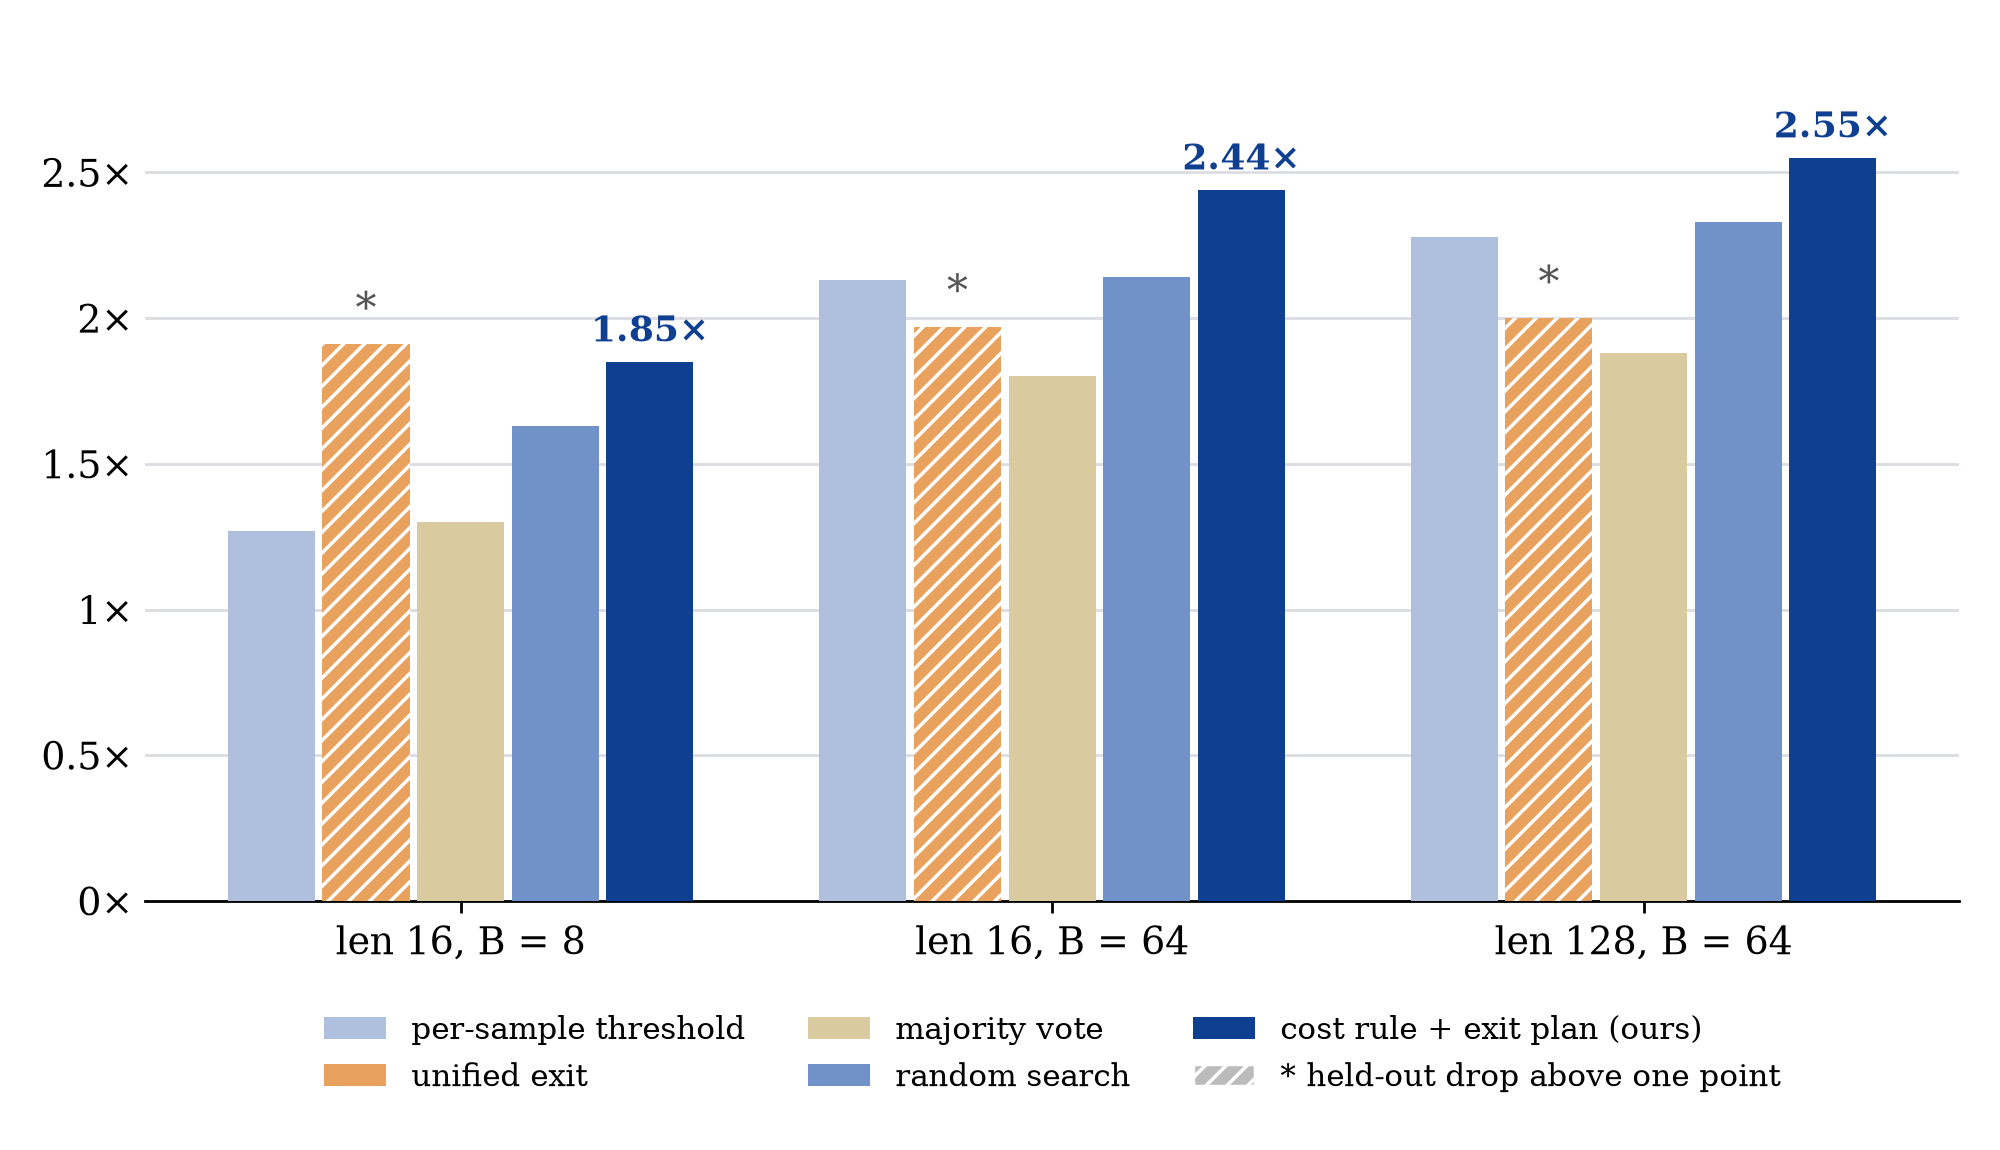
\includegraphics[width=0.78\textwidth]{fig/speedup.png}
  \caption{Speedup over the full model of each method's certified policy, QQP, GTX 1650, timed (values of
  Table~\ref{tab:t04}; chart of the final presentation, redrawn with the over-budget marks of the table).
  Hatched, $^{*}$: held-out drop above one point.}
  \label{fig:speedup}
\end{figure}

\begin{itemize}
  \item The fastest early-exit rule changes with batch size, execution mode and input length; a rule derived from the
  measured per-layer cost tracks it.
  \item At matched held-out accuracy it leads on QQP (2--17\% on the GTX 1650 cost table; 8--14\% timed on the A6000,
  replaying recorded decisions on a random-weight network) and on Llama classifiers with trained weights (3.66\x{}
  against 3.50\x). It has no gain on RoBERTa MNLI or on LLM decoders.
  \item Certified selection keeps the one-point budget on random re-splits (asymptotically); the finite-sample
  certificates are too loose to certify anything at our sample sizes.
  \item The bound on the damage from slowdown inputs is proved for the trimmed collective stop with a fixed active
  set; for the full rule it held empirically in all 25{,}200 batches tested (crafted inputs on CIFAR-100, the hardest
  natural inputs on MNLI and QQP). The label-free bandit has sublinear regret over ten seeds, with no rate claim.
  \item The accuracy loss of any batch-stopping rule lands on hard inputs (2.0--2.7 points on the hardest quarter of
  MNLI).
  \item \textbf{Lesson carried forward.} Search, by an LLM or otherwise, pays off where answers can be checked
  exactly. In early exit, LLM program search only tied our rule. That led us to index coding, where every bound is a
  certificate. The bridge was the Pincer agent (\file{pincer/}, results in \file{docs/PINCER.md}, Section~0, and
  \file{pincer/results/summary\_test2\_b30.md}): on a fresh split of 26 random-family graphs (30\,s per graph, 4-core
  container) its non-LLM policies closed the minrank gap on 13 of 26 graphs against 2 of 26 for the classic pipeline
  (CP-SAT~\cite{cpsat} independent set + TabuCol~\cite{tabucol} clique cover), and its data showed the Kneser pattern
  behind Part~II. An LLM in Pincer's loop did not beat these non-LLM policies.
\end{itemize}
